% CampusCanteen — B.Tech Project Report (BATU Computer Engineering format)
% Compile: pdflatex main.tex (run twice for TOC) or use Overleaf
\documentclass[12pt,a4paper]{report}

\usepackage[utf8]{inputenc}
\usepackage[T1]{fontenc}
\usepackage[margin=1in]{geometry}
\usepackage{mathptmx}
\usepackage{graphicx}
\usepackage{booktabs}
\usepackage{needspace}
\usepackage{float}
\usepackage{fancyhdr}
\usepackage{cite}
\usepackage{hyperref}
\usepackage{enumitem}
\usepackage{listings}
\usepackage{caption}
\usepackage{subcaption}
\usepackage{titlesec}
\usepackage{xcolor}
\usepackage{tikz}
% Shared table formatting — keeps tables within page margins
\usepackage{tabularx}
\usepackage{ragged2e}
\usepackage{array}

\newcolumntype{Y}{>{\raggedright\arraybackslash}X}
\newcolumntype{C}{>{\centering\arraybackslash}X}

% Use inside table environments before tabularx
\newcommand{\tablebodysetup}{\small\setlength{\tabcolsep}{4pt}}


\newcommand{\inr}{Rs.}
\newcommand{\fillme}[1]{\textcolor{red}{\textbf{[FILL: #1]}}}
% =============================================================================
%  Student / official details — CampusCanteen B.Tech report
%  Set \hasimagestrue when screenshots are added to images/
% =============================================================================

\newcommand{\ProjectTitle}{CampusCanteen: Inventory-Aware Smart Canteen Ordering System with Token and QR Pickup}
\newcommand{\ShortTitle}{CampusCanteen}

% --- Official details (group project) ---
\newcommand{\StudentName}{Manoj Shivaji Pawar}
\newcommand{\RollNo}{23030331245027}
\newcommand{\StudentTwoName}{Rameshwar Bappasaheb Naikwade}
\newcommand{\StudentTwoRoll}{23030331245037}
\newcommand{\StudentThreeName}{Sujal Sunil Dombe}
\newcommand{\StudentThreeRoll}{23030331245059}
\newcommand{\CertificateTitle}{\ShortTitle{}: Inventory-Aware Smart Canteen Ordering System with Token and QR Pickup}
\newcommand{\GroupMembers}{%
  \textbf{\StudentName} (\RollNo), %
  \textbf{\StudentTwoName} (\StudentTwoRoll), and %
  \textbf{\StudentThreeName} (\StudentThreeRoll)}
\newcommand{\GroupMembersList}{%
  \begin{tabular}[t]{@{}c@{}}
    \StudentName\ (\RollNo) \\
    \StudentTwoName\ (\StudentTwoRoll) \\
    \StudentThreeName\ (\StudentThreeRoll)
  \end{tabular}}
\newcommand{\ProjectSubtitle}{Inventory-Aware Smart Canteen Ordering with Token and QR Pickup}
\newcommand{\GuideName}{Asst.\ Prof.\ Uzma Munde}
\newcommand{\GuideInitials}{Asst.\ Prof.\ Uzma Munde}
\newcommand{\HODName}{Dr.\ Arwind Kiweleker}
\newcommand{\AcademicYear}{2025--26}

% --- Acknowledgements ---
\newcommand{\AckFamily}{my parents}
\newcommand{\AckFriends}{my friends}

% --- Screenshots: images/01-login.png … 08-staff-verify.png (uploaded) ---
\newif\ifhasimages
\hasimagestrue

\linespread{1.3}

% Header + centered page number only (no footer text)
\pagestyle{fancy}
\fancyhf{}
\lhead{\ShortTitle}
\cfoot{\thepage}
\renewcommand{\headrulewidth}{0.4pt}
\renewcommand{\footrulewidth}{0pt}
\fancypagestyle{plain}{%
  \fancyhf{}%
  \cfoot{\thepage}%
  \renewcommand{\headrulewidth}{0pt}%
  \renewcommand{\footrulewidth}{0pt}%
}
\usetikzlibrary{shapes,arrows,arrows.meta,positioning,fit,shapes.multipart,shapes.geometric}

\titleformat{\chapter}[hang]{\bfseries\fontsize{18}{22}\selectfont}{\thechapter}{1em}{}
\titleformat{name=\chapter,numberless}[block]
  {\centering\bfseries\fontsize{18}{22}\selectfont}
  {}{0pt}{}
\titlespacing*{name=\chapter,numberless}{0pt}{0pt}{1.2em}
\titleformat{\section}{\bfseries\fontsize{16}{19}\selectfont}{\thesection}{1em}{}
\titleformat{\subsection}{\bfseries\fontsize{14}{17}\selectfont}{\thesubsection}{1em}{}

\renewcommand{\contentsname}{Contents}

\captionsetup[figure]{position=bottom,labelfont=bf}
\captionsetup[table]{position=top,labelfont=bf}

\lstset{
  basicstyle=\ttfamily\small,
  breaklines=true,
  frame=single,
  numbers=left,
  numberstyle=\tiny,
}

\hypersetup{colorlinks=true,linkcolor=black,citecolor=black,urlcolor=blue}

\begin{document}

% Front Page
\begin{titlepage}
  \centering
  \vspace*{0.8cm}
  {\fontsize{18}{22}\selectfont\bfseries \ShortTitle\par}
  \vspace{0.5cm}
  {\fontsize{14}{18}\selectfont\itshape Inventory-Aware Smart Canteen Ordering with Token and QR Pickup\par}
  \vspace{0.8cm}
  {\fontsize{16}{20}\selectfont A Project Report\par}
  \vspace{0.6cm}
  {\fontsize{14}{18}\selectfont
    submitted in partial fulfillment of the requirements\\
    for the award of the degree of\\
    Bachelor of Technology\\
    in\\
    COMPUTER ENGINEERING\par}
  \vspace{1cm}
  {\fontsize{14}{18}\selectfont by\par}
  \vspace{0.4cm}
  {\fontsize{14}{18}\selectfont \StudentName\par}
  {\fontsize{14}{18}\selectfont (\RollNo)\par}
  \vspace{0.8cm}
  {\fontsize{14}{18}\selectfont Under the guidance of\par}
  \vspace{0.3cm}
  {\fontsize{14}{18}\selectfont \GuideName\par}
  \vfill
  
\includegraphics[width=2.4cm]{images/batu_logo.jpg}\\[0.5cm]
  {\fontsize{12}{15}\selectfont
    DEPARTMENT OF COMPUTER ENGINEERING\\
    DR. BABASAHEB AMBEDKAR TECHNOLOGICAL UNIVERSITY\\
    Lonere--402103, Tal.\ Mangaon, Dist.\ Raigad (MS) INDIA\par}
  \vspace{0.5cm}
  {\fontsize{14}{18}\selectfont \AcademicYear\par}
\end{titlepage}

% Certificate
\chapter*{Certificate}
\addcontentsline{toc}{chapter}{Certificate}
\vspace{0.5em}
\noindent
The report entitled \textbf{\ProjectTitle} submitted by \textbf{\StudentName} (\RollNo) is approved for the partial fulfillment of the requirement for the award of the degree of Bachelor of Technology in Computer Engineering.
\vspace{2em}

\noindent
\tablebodysetup
\begin{tabularx}{\textwidth}{@{}>{\bfseries}p{0.46\textwidth} >{\bfseries}p{0.46\textwidth}@{}}
  Guide & Head of Department \\
  \GuideInitials & \HODName \\
  Department of Computer Engineering & Department of Computer Engineering \\
\end{tabularx}

\vspace{2em}
\noindent\textbf{Examiners:}
\begin{enumerate}[label=\arabic*.]
  \item \rule{6cm}{0.4pt} \quad (Name: \rule{5cm}{0.4pt})
  \item \rule{6cm}{0.4pt} \quad (Name: \rule{5cm}{0.4pt})
\end{enumerate}

\vspace{1em}
\noindent Place: Dr.\ Babasaheb Ambedkar Technological University, Lonere\\
Date: \ReportDate

% Acknowledgements
\chapter*{Acknowledgements}
\addcontentsline{toc}{chapter}{Acknowledgements}
I would like to express my sincere gratitude to my project guide, \textbf{\GuideName}, for valuable suggestions, regular reviews, and encouragement throughout this work. I am thankful to \textbf{\HODName}, Head of the Department of Computer Engineering, and all faculty members of the department for academic support.

I thank my classmates and \AckFriends, for helpful discussions and testing of the application. I am deeply grateful to \AckFamily, for their constant motivation.

I also acknowledge the open-source communities behind Next.js, Prisma, and related tools that made implementation feasible within the project timeline.

% Abstract
\chapter*{Abstract}
\addcontentsline{toc}{chapter}{Abstract}
\noindent
College canteens serving ready-to-eat food face long queues and overselling when batch-prepared stock is limited. \textbf{\ShortTitle{}} is a web-based, inventory-aware ordering system that lets students browse live menu availability, pre-order items, pay online (simulated gateway for demonstration), and collect food using a pickup token and QR code on a mobile-friendly digital receipt. Canteen staff use the same web application on mobile browsers to manage a pickup queue, mark orders ready, verify QR codes or tokens, confirm handover, update inventory with custom stock quantities (e.g.\ setting exact count to 17 units), and view a demand forecast for next-day preparation.

The system is built with Next.js 16, React 19, TypeScript, Tailwind CSS, Prisma ORM, and PostgreSQL. JWT-based authentication enforces separate student and staff roles. Stock is validated when the cart is reviewed, when an order is created, and when payment is processed; inventory is decremented only after successful payment. The interface is mobile-first and supports progressive web application installation on student and staff phones without a native Android application.

Testing on desktop and mobile browsers confirms end-to-end ordering, stock enforcement, staff verification, and inventory updates. Future work includes real UPI integration, production deployment on HTTPS, automated backups, and refund policies.

\vspace{0.5em}
\noindent\textbf{Keywords:} Smart canteen, inventory management, pre-ordering, QR code verification, pickup token, demand forecasting, progressive web application, Next.js, PostgreSQL.


% ==================== LISTS ====================
\newpage
\tableofcontents
\thispagestyle{plain}
\newpage
\listoffigures
\addcontentsline{toc}{chapter}{List of Figures}
\thispagestyle{plain}
\newpage
\listoftables
\addcontentsline{toc}{chapter}{List of Tables}
\thispagestyle{plain}

% ==================== MAIN BODY ====================
\newpage
\pagenumbering{arabic}
\setcounter{page}{1}
\pagestyle{fancy}

\chapter{Introduction}

\section{Background}
Food service in college canteens differs from restaurant-style delivery platforms. Items such as samosa, vada pav, poha, tea, coffee, and daily specials are typically prepared in batches and kept as ready-to-eat stock at the counter. Students arrive in concentrated bursts between lectures, causing congestion at the ordering and payment points. Manual processes do not communicate real-time stock to students before they join the queue, and staff struggle to coordinate pickups during peak load.

Digital transformation in campuses has increased expectations for mobile-accessible services. A dedicated canteen system must respect batch inventory, minimize counter interaction to pickup only, and provide staff tools for verification and stock control.

\section{Problem Statement}
The following problems motivated this project:
\begin{enumerate}
  \item \textbf{Queue congestion:} Students wait in line to order and pay even when food is already prepared.
  \item \textbf{Overselling:} Orders may be accepted when physical stock is insufficient, causing dissatisfaction.
  \item \textbf{Weak pickup coordination:} Verbal tokens and manual lists are error-prone at busy counters.
  \item \textbf{Untracked cash sales:} Walk-in cash customers reduce stock without updating any digital record unless staff intervene manually.
  \item \textbf{Limited planning data:} Kitchen staff lack simple forecasts for how much to prepare the next day.
\end{enumerate}

\section{Objectives}
The primary objectives of \ShortTitle{} are:
\begin{itemize}
  \item To design and implement a web-based ordering system aligned with batch-prepared canteen inventory.
  \item To enforce stock-aware cart and payment validation and deduct stock only after successful payment.
  \item To generate a unique pickup token and QR-encoded receipt for fast staff verification on mobile devices.
  \item To provide staff modules for queue management, inventory updates including arbitrary stock counts, and demand forecasting.
  \item To deliver a mobile-first progressive web experience installable on phones without developing a native Android application.
\end{itemize}

\section{Scope}
\subsection{In Scope}
Student registration and login; menu with categories and daily special; cart and checkout; simulated digital payment; order receipt with QR; order history and reorder; staff pickup queue; QR and manual token verification; handover confirmation; inventory add/set/sold-out controls; demand forecast dashboard; mobile UI and PWA install guidance.

\subsection{Out of Scope}
Native Android/iOS applications; live UPI/payment gateway (Razorpay, etc.) in the current build; automatic deduction for cash counter sales; post-payment cancellation and automated refunds; multi-canteen franchise support; kitchen display hardware integration.

\section{Proposed Solution Overview}
Students use a browser on their phone to order only items marked available. After payment, they receive token \texttt{A154} style identifiers and a QR code. Staff mark orders ready, scan the QR or type the token, and confirm handover. Inventory staff set exact stock (e.g.\ 17 samosas) or add batch quantities and toggle sold-out status when the counter is empty.

\section{Organization of Report}
Chapter~2 reviews related work. Chapter~3 presents software requirement analysis and module decomposition. Chapter~4 describes software design with DFD and UML diagrams. Chapter~5 specifies software and hardware requirements. Chapter~6 documents implementation and code structure. Chapter~7 concludes and lists future scope. Bibliography and appendices follow.

\section{Report Preparation Note}
Cloud deployment on Vercel with PostgreSQL is documented in the project repository but was intentionally deferred during report preparation to focus on demonstration, testing, and documentation. Local demonstration uses \texttt{npm run dev} on a developer machine with optional Docker-hosted PostgreSQL.

\chapter{Literature Survey / Review of Literature}

\section{Introduction}
This chapter reviews existing approaches to food ordering, inventory control, queue management, QR-based identification, forecasting, and progressive web applications. The review highlights why generic food delivery systems are insufficient for batch-stock college canteens and justifies the design choices of \ShortTitle{}.

\section{Online Food Ordering Platforms}
Platforms such as Swiggy and Zomato optimize restaurant workflows: menu discovery, cart, payment, and delivery or pickup with order-triggered preparation. Research on e-commerce checkout emphasizes cart abandonment reduction and payment trust. However, these systems assume fulfillment capacity is abstracted behind the restaurant---they do not model a visible integer stock that decreases with both online and walk-in sales unless manually updated.

\section{Queue Management Systems}
Queue management literature discusses physical queues, token dispensers, and digital ticketing. Token-based systems reduce perceived waiting time by decoupling ordering from service. Digital tokens displayed on a phone screen extend this model. \ShortTitle{} combines numeric tokens with machine-readable QR payloads to reduce staff typing errors.

\section{Inventory Management}
Retail inventory systems maintain SKU stock, reorder points, and reservations. E-commerce ``only N left'' messaging influences purchase urgency. For canteens, low-stock thresholds trigger labels such as ``Only 5 left'' before sold-out. Critical design decision: validate stock at cart review, order creation, and payment, and decrement only after payment to avoid locking stock for unpaid carts.

\section{QR Codes in Ticketing and Verification}
ISO/IEC 18004 standardizes QR code symbology. Event ticketing and boarding passes use QR for rapid verification. Staff counter cameras on smartphones can decode QR in browsers via \texttt{getUserMedia} and barcode libraries. Pairing QR with a human-readable token provides fallback when scanning fails.

\section{Demand Forecasting}
Hyndman and Athanasopoulos describe time-series forecasting methods. Simple moving averages and weighted historical averages are appropriate when only weeks of sales data exist. \ShortTitle{} uses a 14-day weighted moving average to suggest batch preparation quantities---sufficient for a mini project without requiring deep learning infrastructure.

\section{Progressive Web Applications}
Mozilla and W3C document PWAs: manifest, service worker, installability, and responsive layout. PWAs avoid app store distribution while supporting home-screen icons---aligned with campus deployment constraints and beginner project scope (no native Android development).

\section{Web Application Architecture}
Modern full-stack JavaScript frameworks such as Next.js unify server-rendered pages and API routes, reducing deployment complexity for academic projects. Prisma ORM provides type-safe database access across SQLite (early prototype) and PostgreSQL (production path).

\section{Security and Authentication}
JSON Web Tokens (RFC 7519) in HTTP-only cookies are a common pattern for session management. Role-based access control separates student and staff API surfaces. Password hashing with bcrypt protects stored credentials.

\section{Summary of Research Gap}
Table~\ref{tab:gap} summarizes the gap addressed by this project.

\begin{table}[htbp]
  \centering
  \caption{Comparison with generic food ordering apps}
  \label{tab:gap}
  \tablebodysetup
  \begin{tabularx}{\textwidth}{@{}>{\bfseries}p{0.36\textwidth} C C@{}}
    \toprule
    \textbf{Feature} & \textbf{Generic app} & \textbf{\ShortTitle{}} \\
    \midrule
    Batch stock model & Partial & Central \\
    Custom staff stock count & Rare & Yes (set exact qty.) \\
    QR + token pickup & Varies & Yes \\
    Staff sold-out toggle (cash) & No & Yes \\
    PWA, no native app & Varies & Yes \\
    College forecast module & No & Yes \\
    \bottomrule
  \end{tabularx}
\end{table}

\chapter{Software Requirement Analysis}

\section{Introduction}
This chapter defines the problem in operational terms, identifies stakeholders, and specifies functional and non-functional requirements. Modules are decomposed with responsibilities suitable for implementation in Next.js API routes and React components.

\section{Problem Definition}
The canteen operates with finite ready-to-eat stock. Students should complete ordering and payment before reaching the counter, presenting only a token/QR for pickup. The system must never confirm payment for items that exceed app-tracked stock at payment time. Staff must update stock when physical count differs from the database (e.g.\ exactly 17 samosas remaining) because cash sales are not automatically recorded.

\section{Stakeholders}
\begin{itemize}
  \item \textbf{Student:} Browses menu, pays online, monitors order status, displays QR at pickup.
  \item \textbf{Canteen staff:} Monitors queue, prepares food, verifies pickup, updates inventory.
  \item \textbf{Project guide / examiner:} Evaluates completeness, documentation, and demonstration.
  \item \textbf{College IT (future):} May host HTTPS deployment and database backups.
\end{itemize}

\section{Assumptions and Constraints}
\begin{itemize}
  \item One canteen outlet; single menu list.
  \item Simulated payment acceptable for academic demonstration.
  \item Staff have smartphones with camera for QR scanning.
  \item Internet available on campus Wi-Fi or mobile data.
  \item English UI; currency in Indian Rupees (\inr).
\end{itemize}

\section{Functional Requirements}

\subsection{FR1 -- Authentication}
\begin{itemize}
  \item FR1.1: User shall register with email, name, and optional student ID.
  \item FR1.2: User shall login with email and password.
  \item FR1.3: System shall assign role STUDENT or STAFF and enforce route access.
  \item FR1.4: Session shall persist using secure HTTP-only cookie (JWT).
\end{itemize}

\subsection{FR2 -- Student Menu and Cart}
\begin{itemize}
  \item FR2.1: Display menu with emoji, price, description, category filter.
  \item FR2.2: Show availability: Available, Only N left, Sold out.
  \item FR2.3: Highlight today's special item.
  \item FR2.4: Cart quantity shall not exceed \texttt{stockQuantity}.
  \item FR2.5: Reorder last paid order when items still available.
\end{itemize}

\subsection{FR3 -- Order and Payment}
\begin{itemize}
  \item FR3.1: Validate cart stock via API before review step.
  \item FR3.2: Create order in PENDING state with line items.
  \item FR3.3: Process simulated payment; on success set CONFIRMED and deduct stock.
  \item FR3.4: Generate unique \texttt{orderCode}, \texttt{tokenNumber}, and QR image.
\end{itemize}

\subsection{FR4 -- Pickup and Staff}
\begin{itemize}
  \item FR4.1: List paid orders in staff queue with polling refresh.
  \item FR4.2: Staff marks CONFIRMED $\rightarrow$ READY\_FOR\_PICKUP.
  \item FR4.3: Verify by QR scan or manual token/order code entry.
  \item FR4.4: Confirm handover $\rightarrow$ COMPLETED.
\end{itemize}

\subsection{FR5 -- Inventory}
\begin{itemize}
  \item FR5.1: Staff sets exact \texttt{stockQuantity} (custom count).
  \item FR5.2: Staff adds quantity to existing stock (\texttt{addStock}).
  \item FR5.3: Staff toggles \texttt{isAvailable} for sold-out online.
\end{itemize}

\subsection{FR6 -- Forecast}
\begin{itemize}
  \item FR6.1: Display predicted demand per item and suggested batch size.
  \item FR6.2: Show disclaimer when historical data is limited.
\end{itemize}

\section{Non-Functional Requirements}
\begin{table}[htbp]
  \centering
  \caption{Non-functional requirements}
  \tablebodysetup
  \begin{tabularx}{\textwidth}{@{}l l Y@{}}
    \toprule
    \textbf{ID} & \textbf{Category} & \textbf{Specification} \\
    \midrule
    NFR1 & Usability & Mobile-first; bottom navigation; min.\ touch target 44px \\
    NFR2 & Performance & Menu API cache 8s; poll only when tab visible \\
    NFR3 & Reliability & Stock checks at cart, order, payment \\
    NFR4 & Security & bcrypt passwords; staff-only inventory APIs \\
    NFR5 & Compatibility & Chrome Android, Safari iOS, responsive CSS \\
    NFR6 & Maintainability & TypeScript, modular components, Prisma schema \\
    \bottomrule
  \end{tabularx}
\end{table}

\section{Module Decomposition}
\begin{table}[htbp]
  \centering
  \caption{Modules and functionalities}
  \tablebodysetup
  \begin{tabularx}{\textwidth}{@{}>{\bfseries}p{0.22\textwidth} Y@{}}
    \toprule
    \textbf{Module} & \textbf{Responsibilities} \\
    \midrule
    AuthModule & Login, register, JWT session, role guard \\
    MenuModule & Fetch items, enrich stock labels, daily special \\
    CartModule & Client cart state, validate against server \\
    OrderModule & Create order, status transitions, history \\
    PaymentModule & Simulated pay, stock deduction, token issue \\
    ReceiptModule & QR generation, fullscreen display, polling \\
    QueueModule & Staff list, mark ready, visibility polling \\
    VerifyModule & Parse QR, match order, handover confirm \\
    InventoryModule & PATCH stock, availability toggle \\
    ForecastModule & Aggregate history, weighted average \\
    PWAModule & Manifest, service worker, install UI hints \\
    \bottomrule
  \end{tabularx}
\end{table}

\section{Order Status Rules}
Paid orders progress: \texttt{CONFIRMED} (paid, preparing) $\rightarrow$ \texttt{READY\_FOR\_PICKUP} $\rightarrow$ \texttt{COMPLETED} after verification and handover. \texttt{PENDING} exists only before payment. \texttt{CANCELLED} is reserved for future refund workflows.

\chapter{Software Design}

\section{System Architecture}
The system follows a three-tier architecture: presentation (Next.js React client), application (Next.js API routes), and data (PostgreSQL via Prisma ORM). Figure~\ref{fig:architecture} illustrates the deployment view.

\begin{figure}[htbp]
  \centering
  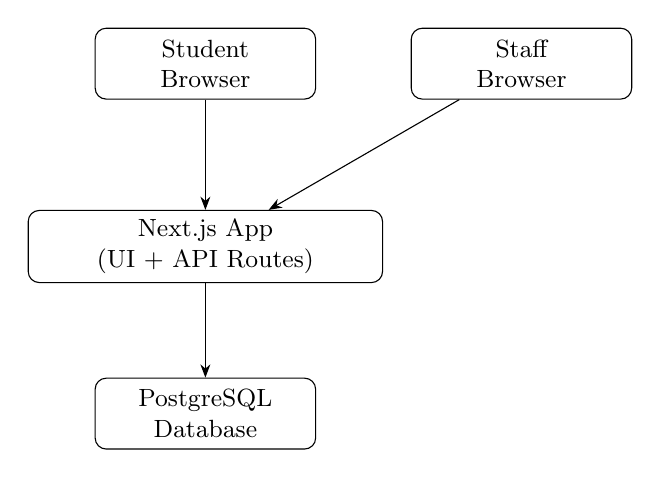
\begin{tikzpicture}[
    box/.style={draw, rounded corners, minimum width=2.8cm, minimum height=0.9cm, align=center, font=\small},
    arr/.style={-{Stealth}}
  ]
    \node[box] (stu) {Student\\Browser};
    \node[box, right=1.2cm of stu] (staff) {Staff\\Browser};
    \node[box, below=1.4cm of stu, minimum width=4.5cm] (next) {Next.js App\\(UI + API Routes)};
    \node[box, below=1.2cm of next] (db) {PostgreSQL\\Database};
    \draw[arr] (stu) -- (next);
    \draw[arr] (staff) -- (next);
    \draw[arr] (next) -- (db);
  \end{tikzpicture}
  \caption{High-level system architecture}
  \label{fig:architecture}
\end{figure}

\section{Data Flow Diagram}
\subsection{Context Diagram (Level 0)}
\begin{figure}[htbp]
  \centering
  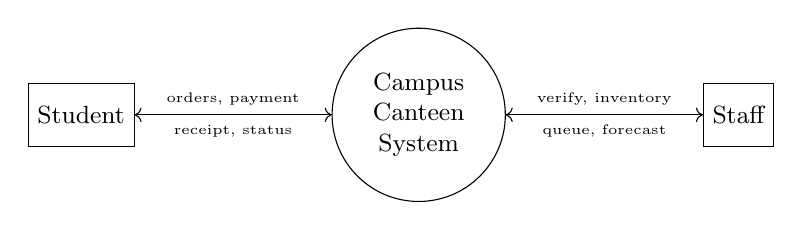
\begin{tikzpicture}[
    proc/.style={draw, circle, minimum size=2.2cm, align=center, font=\small},
    ent/.style={draw, rectangle, minimum height=0.8cm, font=\small}
  ]
    \node[proc] (sys) {Campus\\Canteen\\System};
    \node[ent, left=2.5cm of sys] (s) {Student};
    \node[ent, right=2.5cm of sys] (st) {Staff};
    \draw[->] (s) -- node[above,font=\tiny]{orders, payment} (sys);
    \draw[->] (sys) -- node[below,font=\tiny]{receipt, status} (s);
    \draw[->] (st) -- node[above,font=\tiny]{verify, inventory} (sys);
    \draw[->] (sys) -- node[below,font=\tiny]{queue, forecast} (st);
  \end{tikzpicture}
  \caption{DFD Level 0 (context diagram)}
  \label{fig:dfd0}
\end{figure}

\subsection{Level 1 DFD (Order Placement)}
Figure~\ref{fig:dfd1} decomposes the student ordering path. Staff verification follows a parallel path (queue $\rightarrow$ verify $\rightarrow$ complete).

\begin{figure}[htbp]
  \centering
  \small
  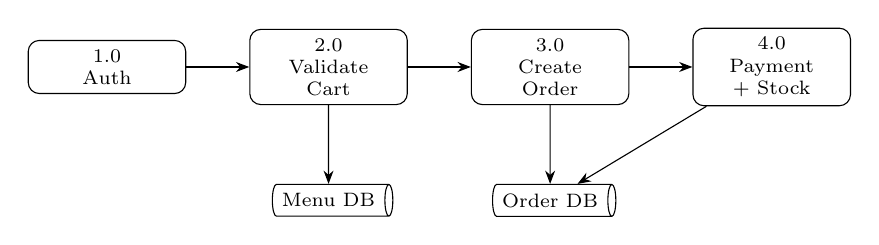
\begin{tikzpicture}[
    proc/.style={draw, rectangle, rounded corners, minimum width=2cm, align=center, font=\scriptsize},
    store/.style={draw, cylinder, shape aspect=0.25, minimum height=0.6cm, font=\scriptsize},
    arr/.style={->, >=Stealth}
  ]
    \node[proc] (auth) {1.0\\Auth};
    \node[proc, right=0.8cm of auth] (val) {2.0\\Validate\\Cart};
    \node[proc, right=0.8cm of val] (ord) {3.0\\Create\\Order};
    \node[proc, right=0.8cm of ord] (pay) {4.0\\Payment\\+ Stock};
    \node[store, below=1cm of val] (d1) {Menu DB};
    \node[store, below=1cm of ord] (d2) {Order DB};
    \draw[arr] (auth) -- (val);
    \draw[arr] (val) -- (ord);
    \draw[arr] (ord) -- (pay);
    \draw[arr] (val) -- (d1);
    \draw[arr] (ord) -- (d2);
    \draw[arr] (pay) -- (d2);
  \end{tikzpicture}
  \caption{DFD Level 1 --- student order and payment (simplified)}
  \label{fig:dfd1}
\end{figure}

\section{UML Use Case Diagram}
\begin{figure}[htbp]
  \centering
  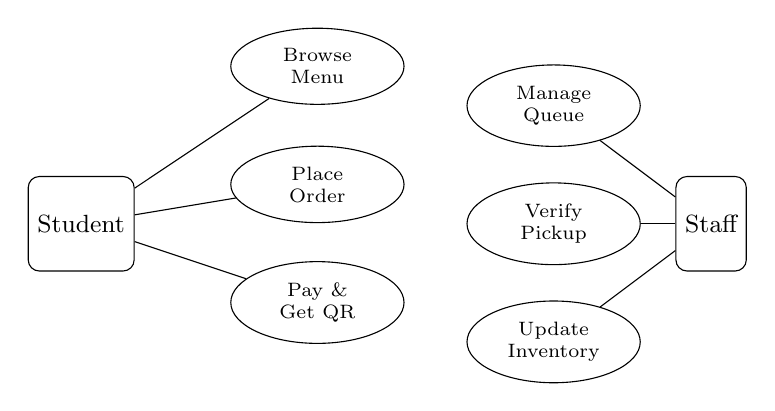
\begin{tikzpicture}[
    actor/.style={draw, shape=rectangle, rounded corners, minimum height=1.2cm, font=\small},
    uc/.style={draw, ellipse, minimum width=2.2cm, minimum height=0.7cm, font=\scriptsize, align=center}
  ]
    \node[actor] (student) at (-4,0) {Student};
    \node[actor] (staff) at (4,0) {Staff};
    \node[uc] (browse) at (-1,2) {Browse\\Menu};
    \node[uc] (order) at (-1,0.5) {Place\\Order};
    \node[uc] (pay) at (-1,-1) {Pay \&\\Get QR};
    \node[uc] (queue) at (2,1.5) {Manage\\Queue};
    \node[uc] (verify) at (2,0) {Verify\\Pickup};
    \node[uc] (inv) at (2,-1.5) {Update\\Inventory};
    \draw (student) -- (browse);
    \draw (student) -- (order);
    \draw (student) -- (pay);
    \draw (staff) -- (queue);
    \draw (staff) -- (verify);
    \draw (staff) -- (inv);
  \end{tikzpicture}
  \caption{Use case diagram}
  \label{fig:usecase}
\end{figure}

\section{UML Class Diagram}
\begin{figure}[htbp]
  \centering
  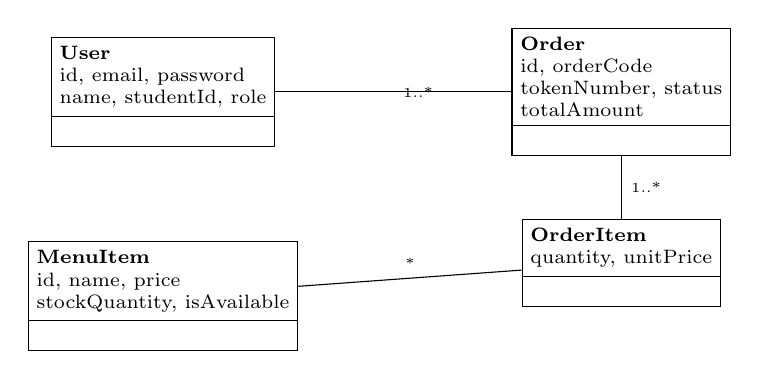
\begin{tikzpicture}[
    class/.style={draw, rectangle split, rectangle split parts=2, align=left, font=\scriptsize, inner sep=3pt}
  ]
    \node[class] (user) {\textbf{User}\\id, email, password\\name, studentId, role};
    \node[class, below=1.2cm of user] (menu) {\textbf{MenuItem}\\id, name, price\\stockQuantity, isAvailable};
    \node[class, right=3cm of user] (order) {\textbf{Order}\\id, orderCode\\tokenNumber, status\\totalAmount};
    \node[class, below=0.8cm of order] (oi) {\textbf{OrderItem}\\quantity, unitPrice};
    \draw (user) -- node[right,font=\tiny]{1..*} (order);
    \draw (order) -- node[right,font=\tiny]{1..*} (oi);
    \draw (menu) -- node[above,font=\tiny]{*} (oi);
  \end{tikzpicture}
  \caption{Simplified class diagram (domain models)}
  \label{fig:class}
\end{figure}

\section{Interaction Diagrams (Sequence / Collaboration)}
The payment and pickup flow involves four collaborators: Student browser, Next.js client, API server, and Staff browser. Figure~\ref{fig:sequence} lists message order equivalent to a UML sequence diagram. Collaboration view emphasizes the same messages grouped by object boundary without temporal ordering detail.

\section{Sequence Diagram (Payment and Pickup)}
\begin{figure}[htbp]
  \centering
  \tablebodysetup
  \begin{tabularx}{\textwidth}{@{}Y@{}}
    \textbf{Actors:} Student browser, Next.js client, API server, Staff browser.\\
    \textit{1. POST /api/cart/validate}\\
    \textit{2. POST /api/orders $\rightarrow$ PENDING}\\
    \textit{3. POST /api/payments $\rightarrow$ CONFIRMED, stock deducted}\\
    \textit{4. GET /api/orders/\{id\}/qr}\\
    \textit{5. Staff: mark ready $\rightarrow$ READY\_FOR\_PICKUP}\\
    \textit{6. POST /api/orders/verify (QR or token)}\\
    \textit{7. POST confirm-handover $\rightarrow$ COMPLETED}\\
  \end{tabularx}
  \caption{Sequence of operations for order payment and pickup (tabular form)}
  \label{fig:sequence}
\end{figure}

\section{Order State Diagram}
\begin{figure}[htbp]
  \centering
  
\begin{tikzpicture}[
    st/.style={draw, rounded corners, font=\small},
    arr/.style={-{Stealth}}
  ]
    \node[st] (p) {PENDING};
    \node[st, right=1.5cm of p] (c) {CONFIRMED};
    \node[st, right=1.5cm of c] (r) {READY};
    \node[st, right=1.5cm of r] (d) {COMPLETED};
    \draw[arr] (p) -- node[above,font=\tiny]{pay} (c);
    \draw[arr] (c) -- node[above,font=\tiny]{pack} (r);
    \draw[arr] (r) -- node[above,font=\tiny]{handover} (d);
  \end{tikzpicture}
  \caption{Control flow / order status states}
  \label{fig:states}
\end{figure}

\section{Database Design (E-R Diagram)}
\begin{figure}[htbp]
  \centering
  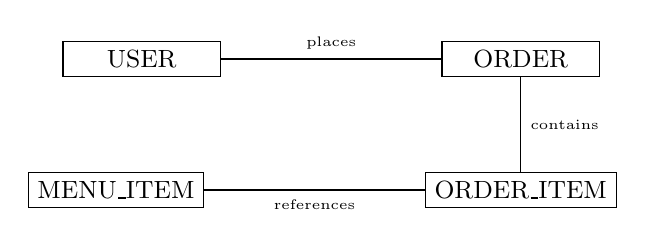
\begin{tikzpicture}[
    ent/.style={draw, rectangle, minimum width=2cm, align=center, font=\small}
  ]
    \node[ent] (u) {USER};
    \node[ent, right=2.8cm of u] (o) {ORDER};
    \node[ent, below=1.2cm of o] (oi) {ORDER\_ITEM};
    \node[ent, left=2.8cm of oi] (m) {MENU\_ITEM};
    \draw (u) -- node[above,font=\tiny]{places} (o);
    \draw (o) -- node[right,font=\tiny]{contains} (oi);
    \draw (m) -- node[below,font=\tiny]{references} (oi);
  \end{tikzpicture}
  \caption{Entity--relationship diagram}
  \label{fig:er}
\end{figure}

\section{Table Schema Summary}
Table~\ref{tab:entities} lists the four database entities and key fields (Prisma schema).

\Needspace{14\baselineskip}
\begin{table}[H]
  \centering
  \caption{Primary entities and key attributes}
  \label{tab:entities}
  \scriptsize
  \setlength{\tabcolsep}{4pt}
  \renewcommand{\arraystretch}{1.12}
  \begin{tabularx}{0.88\textwidth}{@{}>{\bfseries}p{0.14\textwidth} >{\raggedright\arraybackslash}X@{}}
    \toprule
    Entity & Key attributes \\
    \midrule
    User & id, email, name, password, role, studentId, createdAt \\
    MenuItem & id, name, description, price, category, stockQuantity, lowStockThreshold, isAvailable, isDailySpecial \\
    Order & id, orderCode, tokenNumber, orderNumber, userId, status, paymentStatus, totalAmount, createdAt \\
    OrderItem & id, orderId, menuItemId, quantity, unitPrice \\
    \bottomrule
  \end{tabularx}
\end{table}

\chapter{Software and Hardware Requirements}

\section{Introduction}
This chapter lists software and hardware needed for development, demonstration, and future production deployment of \ShortTitle{}.

\section{Software Requirements}

\subsection{Development Tools}
\begin{table}[htbp]
  \centering
  \caption{Development software}
  \tablebodysetup
  \begin{tabularx}{\textwidth}{@{}l Y@{}}
    \toprule
    \textbf{Software} & \textbf{Version / note} \\
    \midrule
    Node.js & 18.x or 20.x LTS \\
    npm & Bundled with Node.js \\
    Next.js & 16.x (App Router) \\
    React & 19.x \\
    TypeScript & 5.x \\
    Prisma CLI & 6.x \\
    PostgreSQL & 16 (Docker or Neon) \\
    Git & Latest \\
    VS Code / Cursor & Editor \\
    Chrome DevTools & Mobile emulation, network throttling \\
    \LaTeX{} & TeX Live or Overleaf (this report) \\
    \bottomrule
  \end{tabularx}
\end{table}

\subsection{Runtime Dependencies (npm)}
Key libraries: \texttt{@prisma/client}, \texttt{bcryptjs}, \texttt{jose} (JWT), \texttt{qrcode}, \texttt{html5-qrcode}, \texttt{recharts}, \texttt{zod}, \texttt{date-fns}, \texttt{lucide-react}, \texttt{tailwindcss}.

\subsection{Browser Requirements (End Users)}
\begin{itemize}
  \item \textbf{Student:} Modern mobile browser; JavaScript enabled.
  \item \textbf{Staff:} Chrome or Brave on Android recommended for QR camera; Safari on iOS supported with manual token fallback.
  \item \textbf{PWA install:} HTTPS in production; on LAN HTTP demo, manual ``Add to Home screen'' instructions shown.
\end{itemize}

\subsection{Environment Variables}
\begin{table}[htbp]
  \centering
  \caption{Configuration variables}
  \tablebodysetup
  \begin{tabularx}{\textwidth}{@{}l Y@{}}
    \toprule
    \textbf{Variable} & \textbf{Purpose} \\
    \midrule
    DATABASE\_URL & PostgreSQL connection string \\
    JWT\_SECRET & Signing key for session tokens \\
    NODE\_ENV & development / production \\
    \bottomrule
  \end{tabularx}
\end{table}

\section{Hardware Requirements}

\subsection{Developer Machine}
\begin{itemize}
  \item CPU: Intel Core i3 or equivalent (multi-core recommended).
  \item RAM: 8 GB minimum; 16 GB recommended for Node.js and browser testing.
  \item Storage: 3 GB free (node\_modules, database, build artifacts).
  \item Display: 1920$\times$1080 helpful for DevTools mobile preview.
\end{itemize}

\subsection{Demonstration Setup (Viva)}
\begin{itemize}
  \item One laptop running development server (\texttt{npm run dev}, port 3000).
  \item Two smartphones (or one phone + laptop) for student and staff roles.
  \item Wi-Fi router allowing devices on same subnet.
  \item Optional: Docker Desktop for local PostgreSQL container.
\end{itemize}

\subsection{Future Production Server}
Cloud hosting (e.g.\ Vercel serverless functions) does not require college-owned server hardware; managed PostgreSQL (Neon, Vercel Postgres) provides database hardware. Estimated concurrent users for mini project: 50--100 simultaneous browser sessions before requiring scaling review.

\section{Network Requirements}
\begin{itemize}
  \item Local demo: firewall allows inbound TCP port 3000 on laptop; phones use \texttt{http://<laptop-IP>:3000}.
  \item Production: HTTPS TLS 1.2+; stable outbound internet for hosting provider.
  \item Slow network: client uses 20s fetch timeout and offline detection banner.
\end{itemize}

\section{Data Storage Requirements}
PostgreSQL database size for one semester demo: $<$ 100 MB (users, orders, menu). Backup policy in production: daily automated snapshots (future work).

\chapter{Coding / Implementation}

\section{Introduction}
This chapter describes the implementation of \ShortTitle{} including technology choices, directory structure, major classes/modules, API design, and representative algorithms. The complete source code is available in the project repository folder \texttt{canteen-preorder/}.

\section{Technology Stack}
\begin{table}[H]
  \centering
  \caption{Implementation stack}
  \tablebodysetup
  \begin{tabularx}{\textwidth}{@{}l Y@{}}
    \toprule
    \textbf{Layer} & \textbf{Technology} \\
    \midrule
    Frontend & React 19, Next.js 16 App Router, Tailwind CSS 4 \\
    Backend & Next.js API Routes (serverless-ready) \\
    ORM & Prisma 6 \\
    Database & PostgreSQL (Docker locally; cloud for deploy) \\
    Auth & JWT (jose), bcryptjs password hash \\
    QR & qrcode (generate), html5-qrcode + BarcodeDetector (scan) \\
    Charts & Recharts (staff forecast) \\
    Validation & Zod (API request bodies) \\
    \bottomrule
  \end{tabularx}
\end{table}

\section{Directory Structure}
\begin{lstlisting}[caption={Project layout (abbreviated)}]
canteen-preorder/
  prisma/schema.prisma      -- User, MenuItem, Order, OrderItem
  prisma/seed.ts            -- Demo accounts and menu
  src/app/api/              -- REST endpoints
  src/components/           -- StudentApp, StaffApp, UI
  src/components/student/   -- Mobile menu, cart sheet, nav
  src/components/staff/     -- Queue, inventory, forecast
  src/lib/                  -- auth, inventory, qr, fetch-client
  public/manifest.webmanifest
  public/sw.js              -- Service worker (PWA)
  docs/batu-project-report/ -- This LaTeX report
\end{lstlisting}

\section{Database Schema Implementation}
Prisma models implement the E-R design: \texttt{User} (role enum), \texttt{MenuItem} (stock fields), \texttt{Order} (token, status enums), \texttt{OrderItem} (line quantities). Enums \texttt{OrderStatus} and \texttt{PaymentStatus} enforce valid transitions at the application layer.

\section{API Implementation Summary}
Each route validates session role via \texttt{requireSession}. Table~\ref{tab:api} lists endpoints.

\begin{table}[H]
  \centering
  \caption{API endpoints}
  \label{tab:api}
  \tablebodysetup
  \begin{tabularx}{\textwidth}{@{}l l Y@{}}
    \toprule
    \textbf{HTTP} & \textbf{Path} & \textbf{Description} \\
    \midrule
    POST & /api/auth & Login / register \\
    GET & /api/auth/session & Current user \\
    GET & /api/menu & Menu + daily special + stock labels \\
    POST & /api/cart/validate & Stock validation for cart \\
    POST & /api/orders & Create PENDING order \\
    GET & /api/orders & Student order history \\
    POST & /api/payments & Pay; deduct stock; CONFIRMED \\
    GET & /api/orders/[id]/qr & QR data URL \\
    GET & /api/orders/queue & Staff queue \\
    POST & /api/orders/verify & Verify token/QR \\
    POST & /api/orders/[id]/confirm-handover & COMPLETED \\
    PATCH & /api/inventory & Stock / availability update \\
    GET & /api/forecast & Demand forecast JSON \\
    \bottomrule
  \end{tabularx}
\end{table}

\section{Module Descriptions}

\subsection{Authentication (\texttt{src/lib/auth.ts})}
\textbf{Purpose:} Issue and verify JWT stored in HTTP-only cookie \texttt{session}.

\textbf{Methods:}
\begin{itemize}
  \item \texttt{createSession(user)} --- Input: user record; Output: Set-Cookie header.
  \item \texttt{getSession()} --- Input: request cookies; Output: payload or null.
  \item \texttt{requireSession(roles[])} --- Input: allowed roles; Output: user or 401/403.
\end{itemize}

\subsection{Inventory (\texttt{src/lib/inventory.ts})}
\textbf{Purpose:} Business rules for stock display and mutation.

\textbf{Methods:}
\begin{itemize}
  \item \texttt{getStockStatus(qty, threshold)} $\rightarrow$ \texttt{available|low|out}.
  \item \texttt{enrichMenuItem(row)} $\rightarrow$ adds \texttt{canOrder}, \texttt{availabilityLabel}.
  \item \texttt{validateCartItems(lines)} $\rightarrow$ array of errors or valid flag.
  \item \texttt{deductStockForOrder(orderId)} $\rightarrow$ transactional decrement per line.
\end{itemize}

\subsection{Student Application (\texttt{StudentApp.tsx})}
\textbf{Purpose:} Single-page student workflow with steps \texttt{menu}, \texttt{review}, \texttt{payment}, \texttt{receipt}.

\textbf{Key state variables:} \texttt{cart}, \texttt{step}, \texttt{pendingOrder}, \texttt{paidOrder}, \texttt{mobileTab}.

\textbf{Features:} Category filter, bottom cart bar, mobile cart sheet, checkout step bar (compact on mobile), active order banner, visibility-aware polling (\texttt{useVisibilityPolling}), toast on add-to-cart.

\subsection{Staff Application (\texttt{StaffApp.tsx})}
\textbf{Purpose:} Tabbed staff UI: queue, verify (QR scanner), inventory, forecast.

\textbf{Inventory PATCH body:}
\begin{lstlisting}[caption={Custom stock update examples}]
{ "menuItemId": "...", "stockQuantity": 17 }  // set exact count
{ "menuItemId": "...", "addStock": 30 }       // add to current
{ "menuItemId": "...", "isAvailable": false } // sold out online
\end{lstlisting}

\subsection{QR Library (\texttt{src/lib/qr.ts})}
Encodes order ID and verification fields in QR payload. \texttt{parseQrPayload} and \texttt{verifyPayloadBody} normalize scanner output for \texttt{/api/orders/verify}.

\subsection{Forecast (\texttt{src/lib/forecast.ts})}
Aggregates completed orders over 14 days, computes weighted moving average per menu item, outputs \texttt{suggestedPrep} and trend indicator (up/down/stable).

\section{User Interface Components}
The main React components used in the student and staff interfaces are listed in Table~\ref{tab:ui-components}.

\begin{table}[H]
  \centering
  \caption{Major UI components}
  \label{tab:ui-components}
  \tablebodysetup
  \begin{tabularx}{\textwidth}{@{}l Y@{}}
    \toprule
    \textbf{Component} & \textbf{Role} \\
    \midrule
    MenuItemRow & Compact menu line with +/- controls \\
    BottomCartBar / MobileCartSheet & Mobile checkout entry \\
    OrderReceipt / FullscreenQrModal & Token + QR display \\
    StaffTabBar & Horizontal staff navigation \\
    InventoryStockControls & Add / Set to / +10 / +25 \\
    PwaInstallPanel & Install instructions per platform \\
    NetworkStatusBanner & Offline user feedback \\
    \bottomrule
  \end{tabularx}
\end{table}

\section{Algorithms}

\subsection{Stock Validation (Cart)}
For each cart line, fetch menu item; if \texttt{!isAvailable} or \texttt{quantity > stockQuantity}, append error with message; return HTTP 409 if any error.

\subsection{Payment and Stock Deduction}
On successful payment API: verify order PENDING; re-validate stock; update order to PAID/CONFIRMED; assign token; call \texttt{deductStockForOrder}; return order JSON for receipt view.

\subsection{Token Generation}
Unique \texttt{tokenNumber} (e.g.\ A154) and \texttt{orderCode} (e.g.\ ORD-2026-54) generated at payment time with collision checks against database unique constraints.

\section{Screenshots of the Developed System}
\label{sec:ui-screenshots}
Figures~\ref{fig:login}--\ref{fig:staff-verify} show the main screens of \ShortTitle{} captured from the running application on a mobile viewport.

% UI screenshots — include from chapter06-coding.tex
% Requires images/*.png and \hasimagestrue in student-info.tex

\ifhasimages

\begin{figure}[htbp]
  \centering
  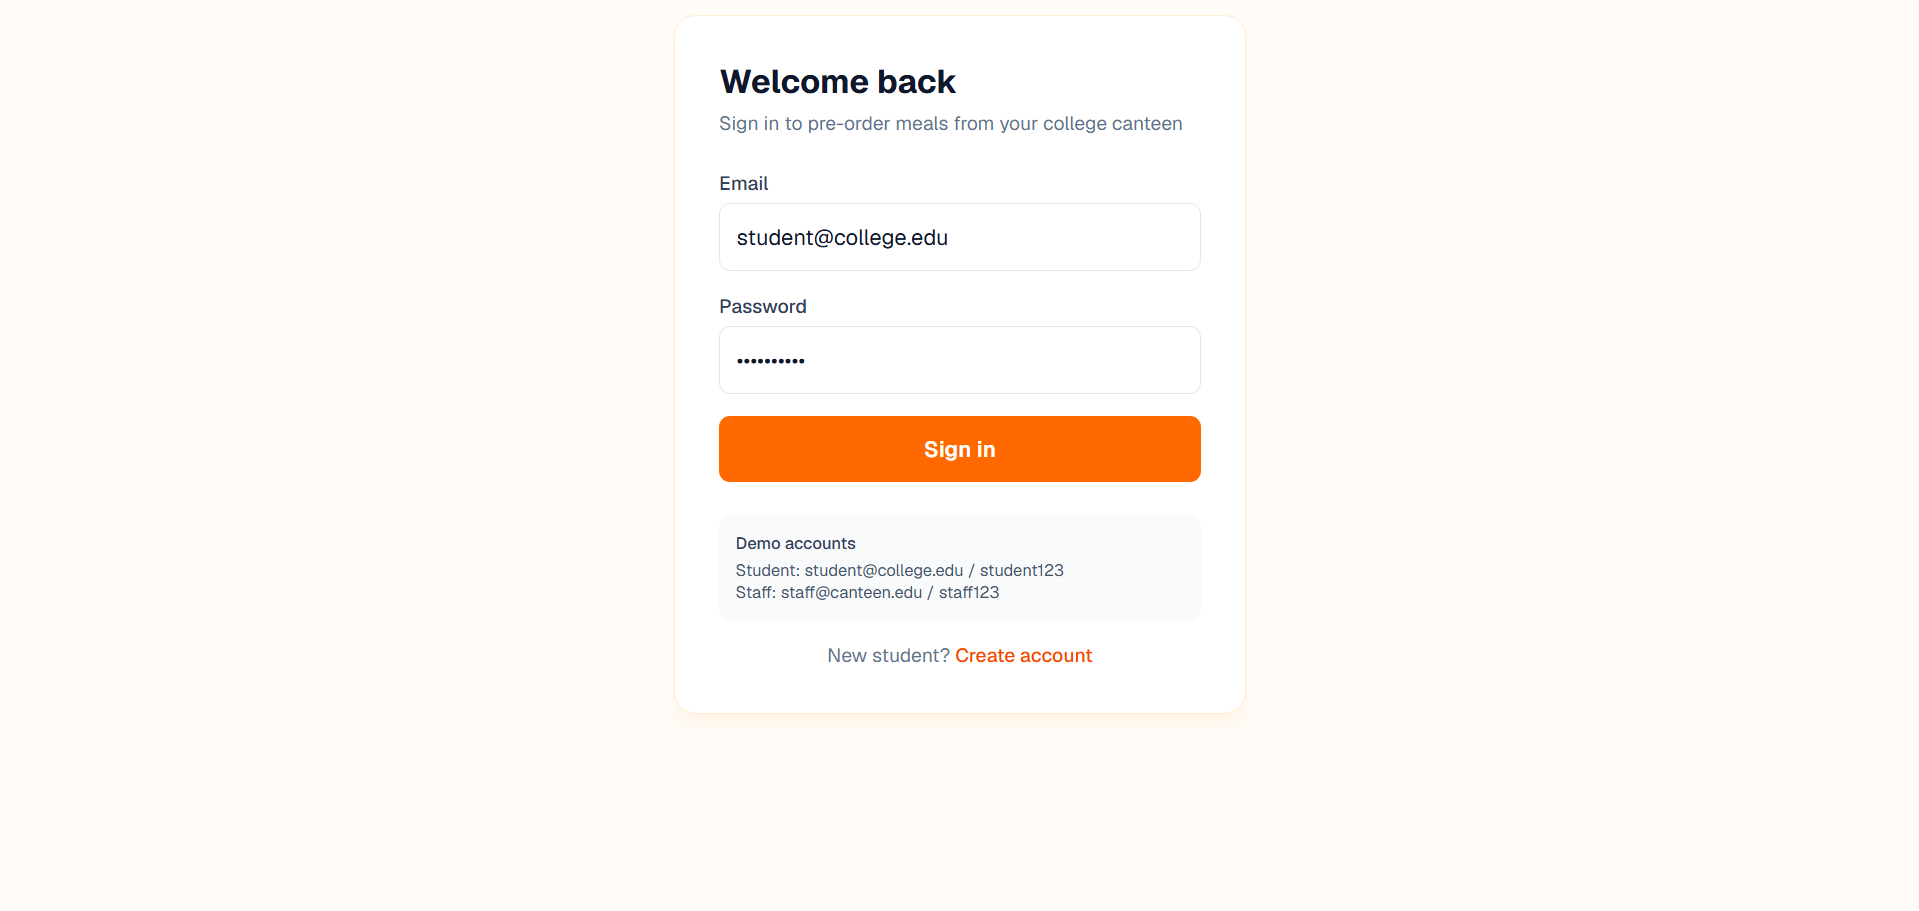
\includegraphics[width=0.85\textwidth]{images/01-login.png}
  \caption{Login page --- student and staff credentials}
  \label{fig:login}
\end{figure}

\begin{figure}[htbp]
  \centering
  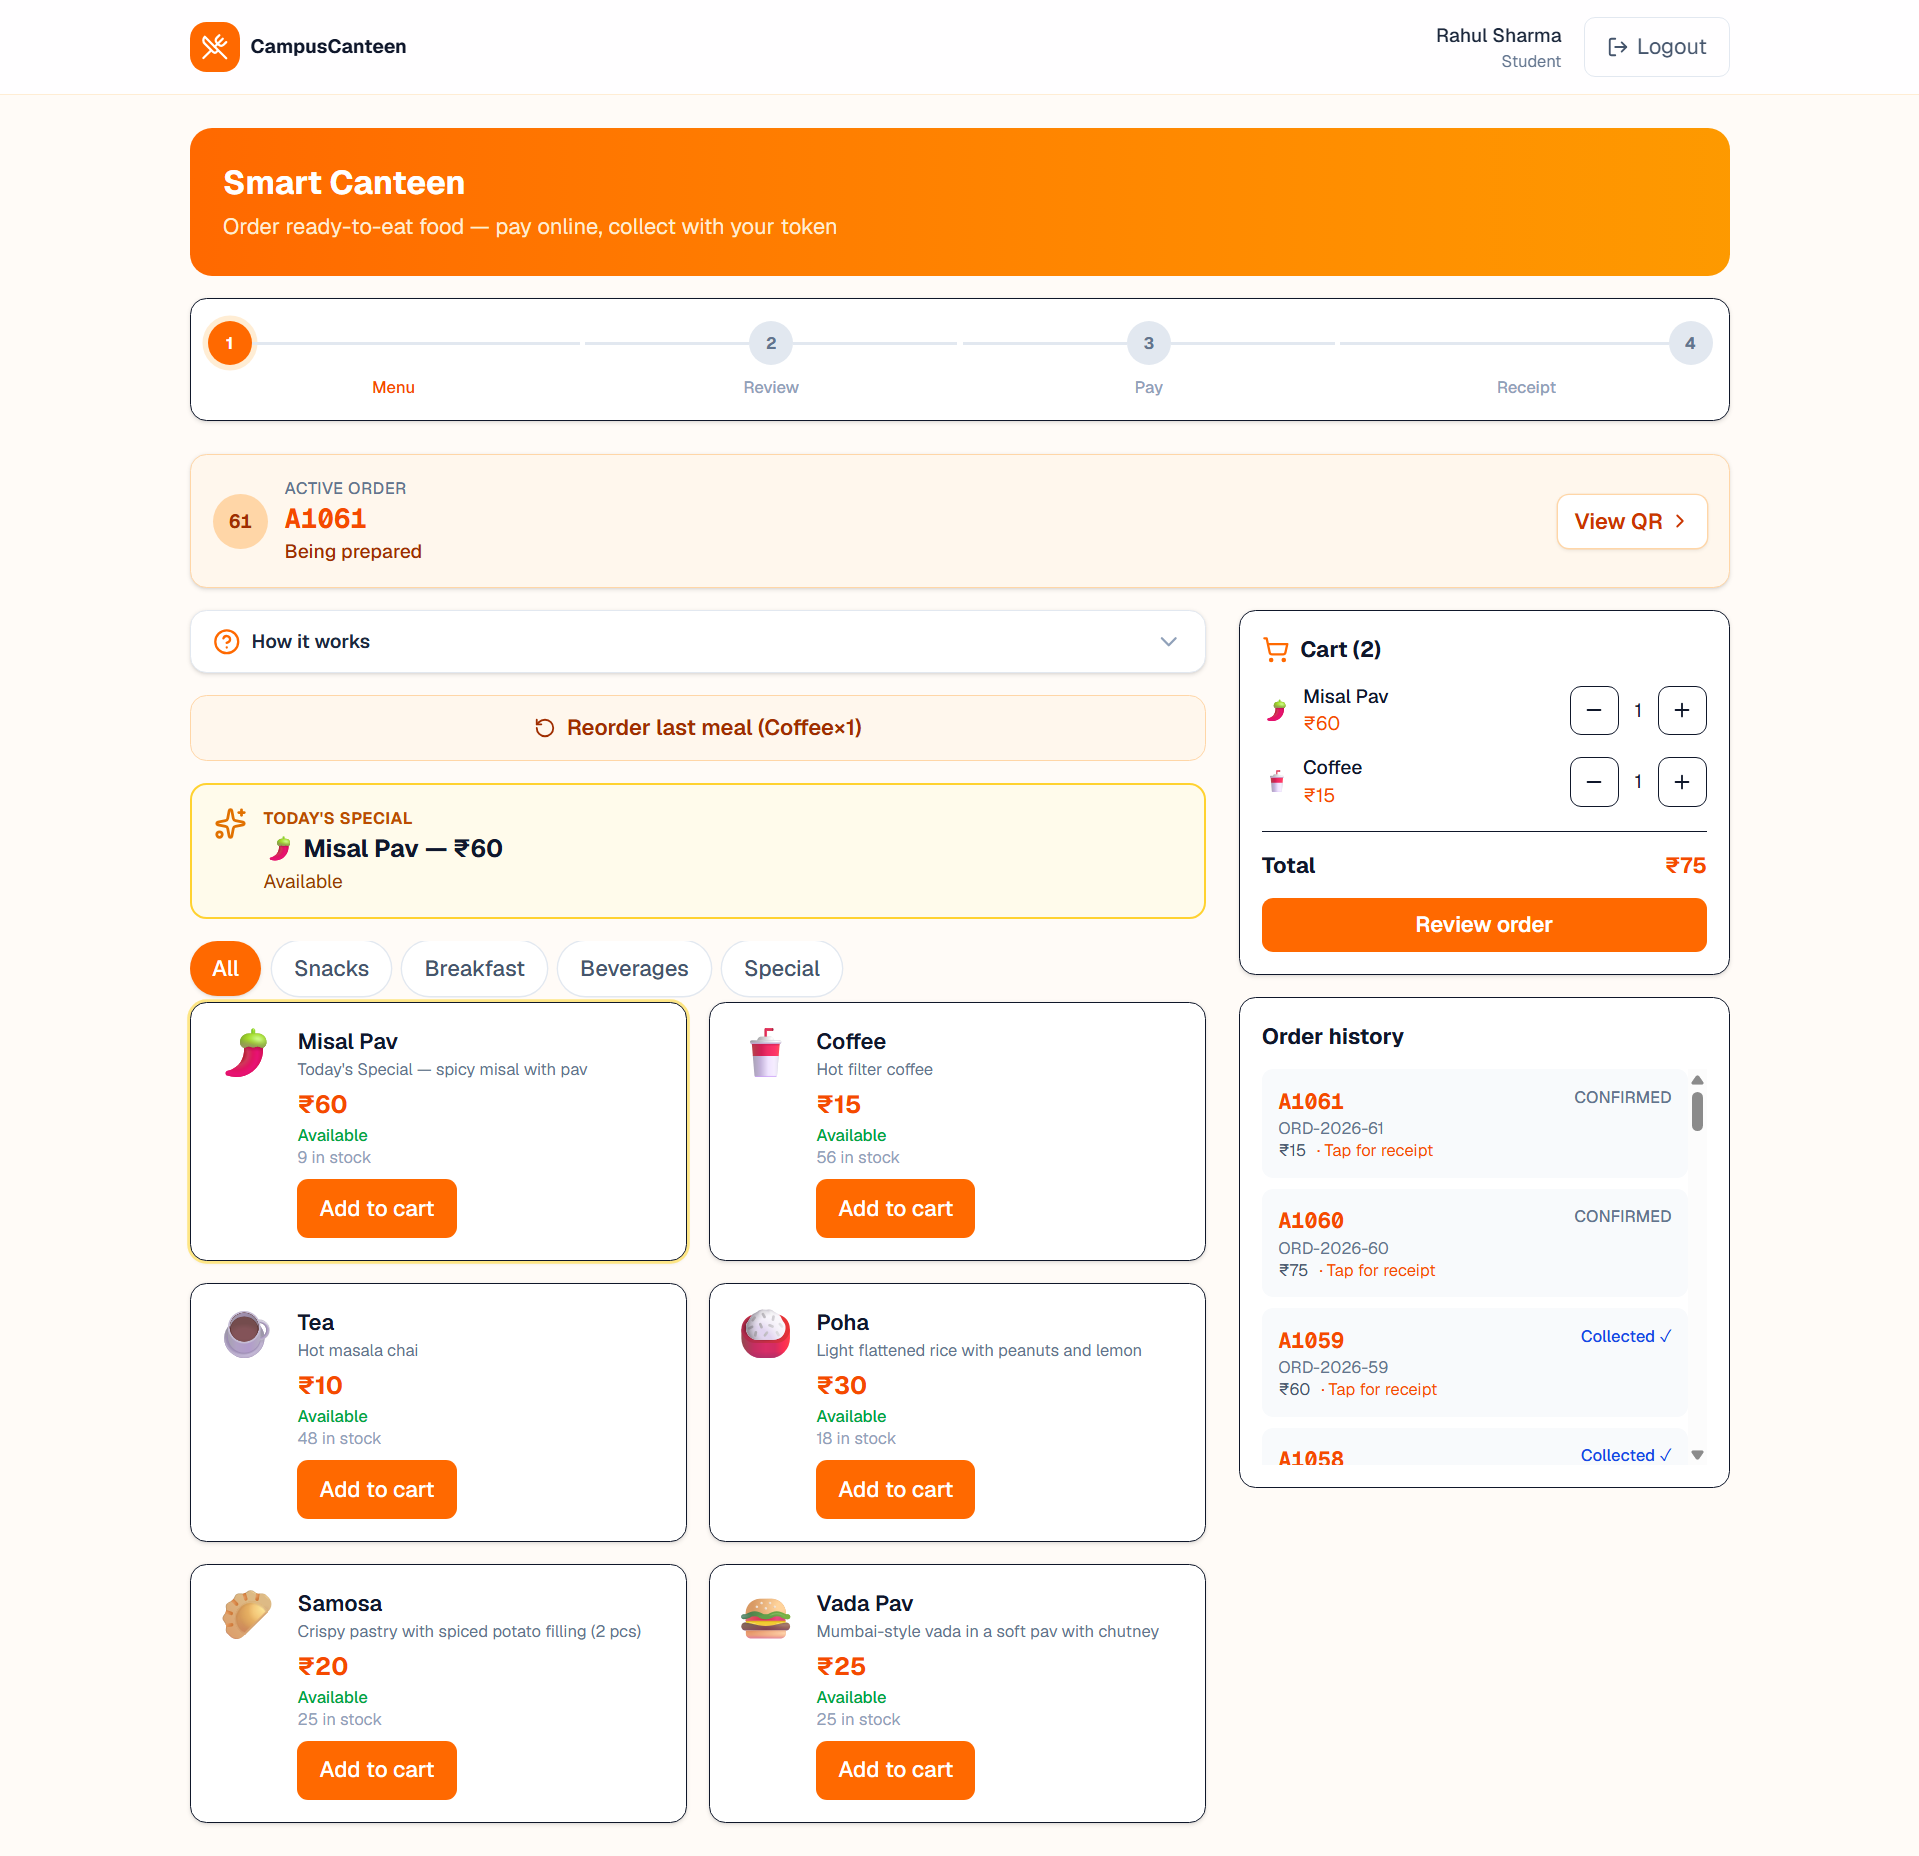
\includegraphics[width=0.85\textwidth]{images/02-student-menu.png}
  \caption{Student menu screen (mobile layout) with categories and stock labels}
  \label{fig:student-menu}
\end{figure}

\begin{figure}[htbp]
  \centering
  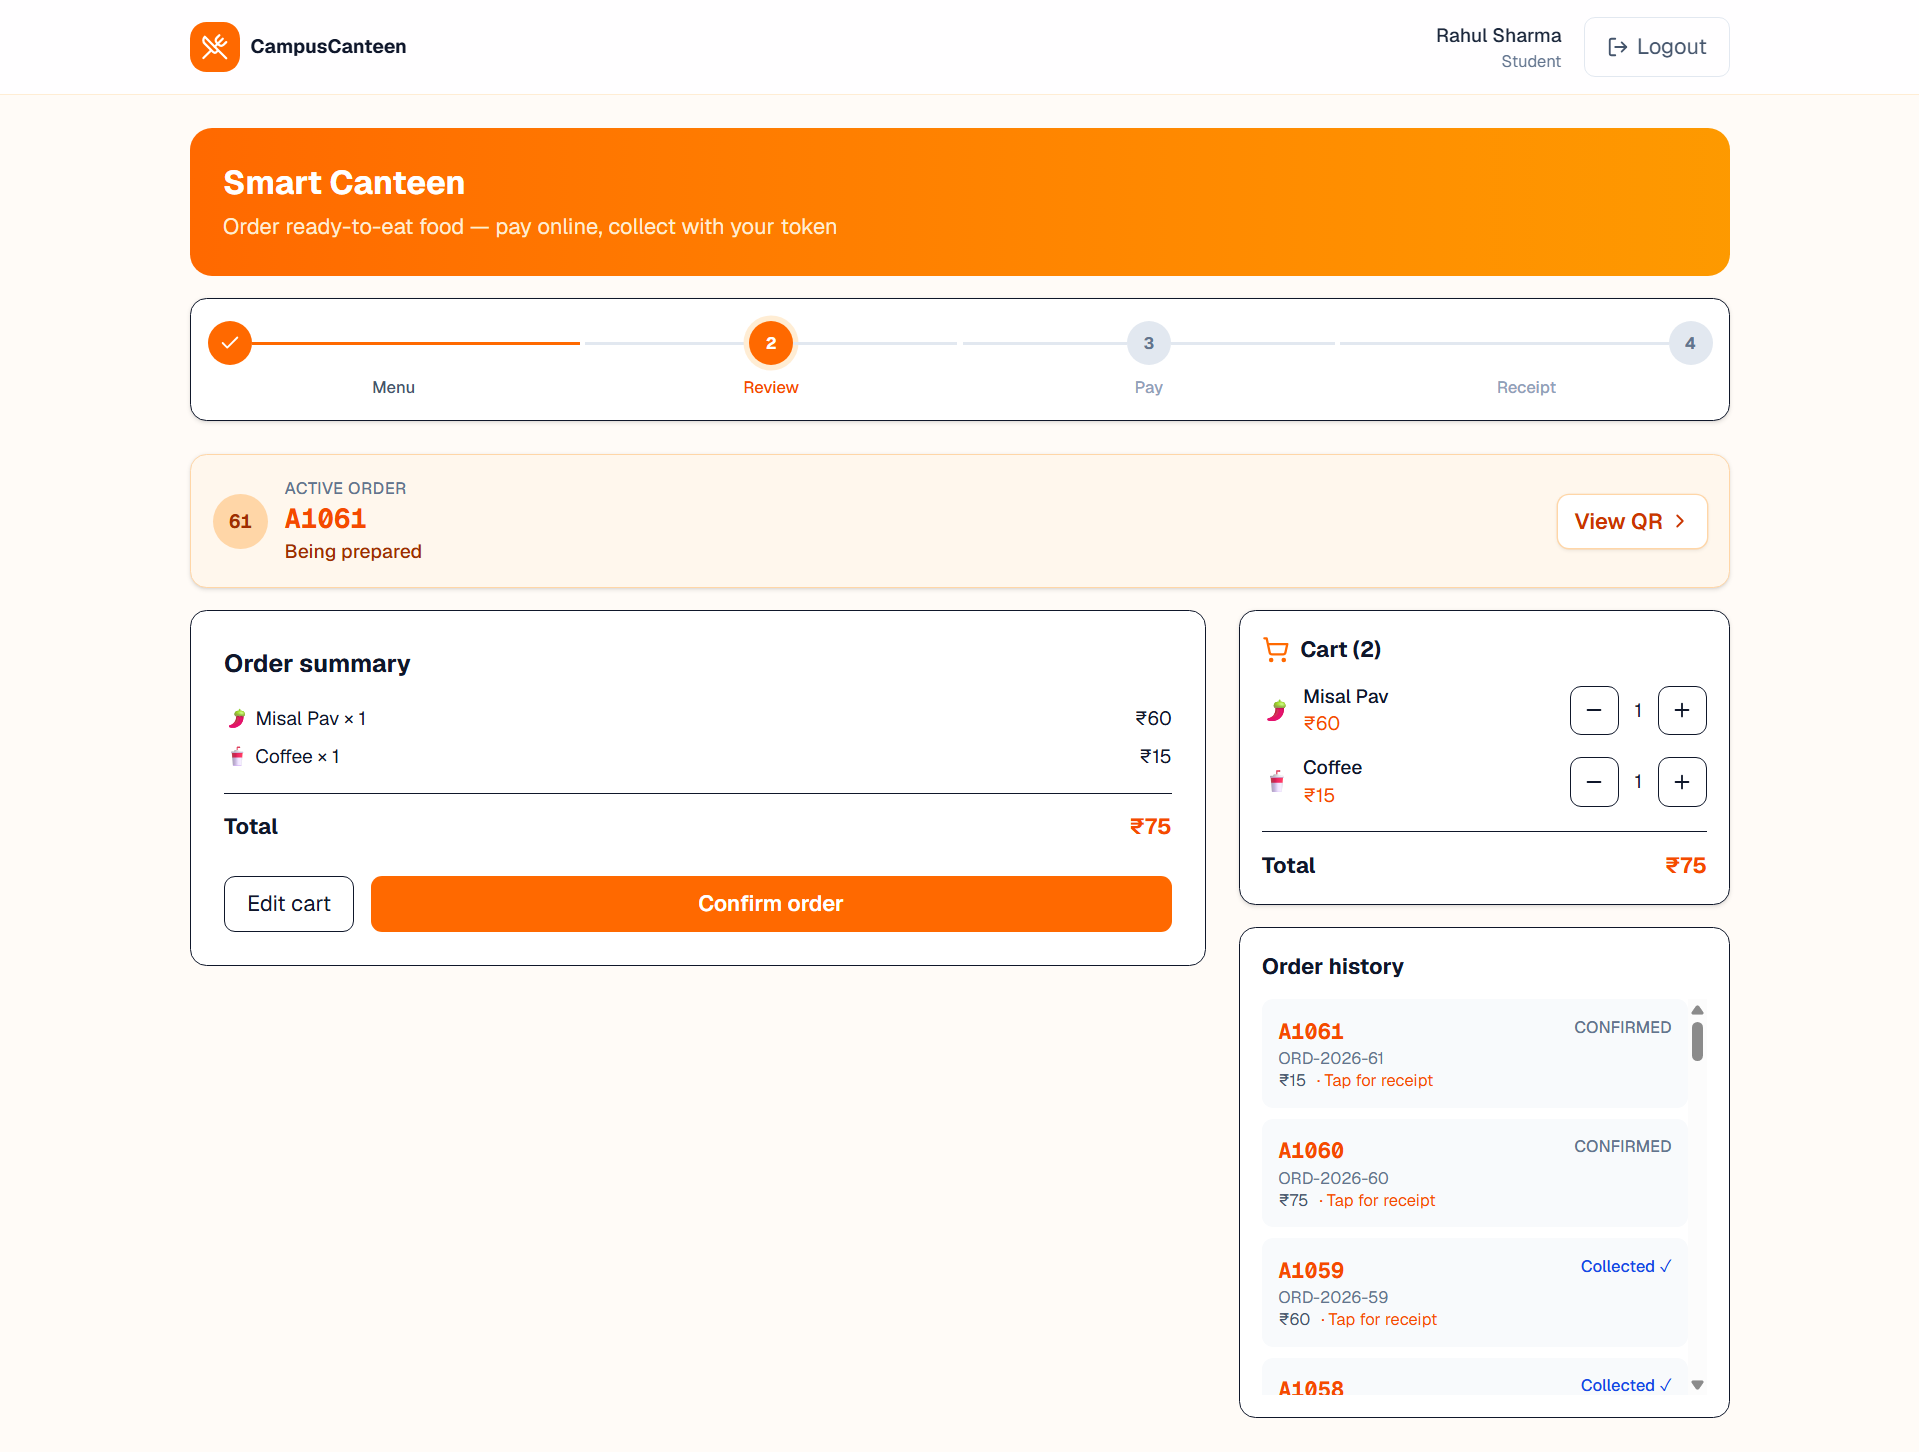
\includegraphics[width=0.85\textwidth]{images/03-review-order.png}
  \caption{Order review step before payment}
  \label{fig:review-order}
\end{figure}

\begin{figure}[htbp]
  \centering
  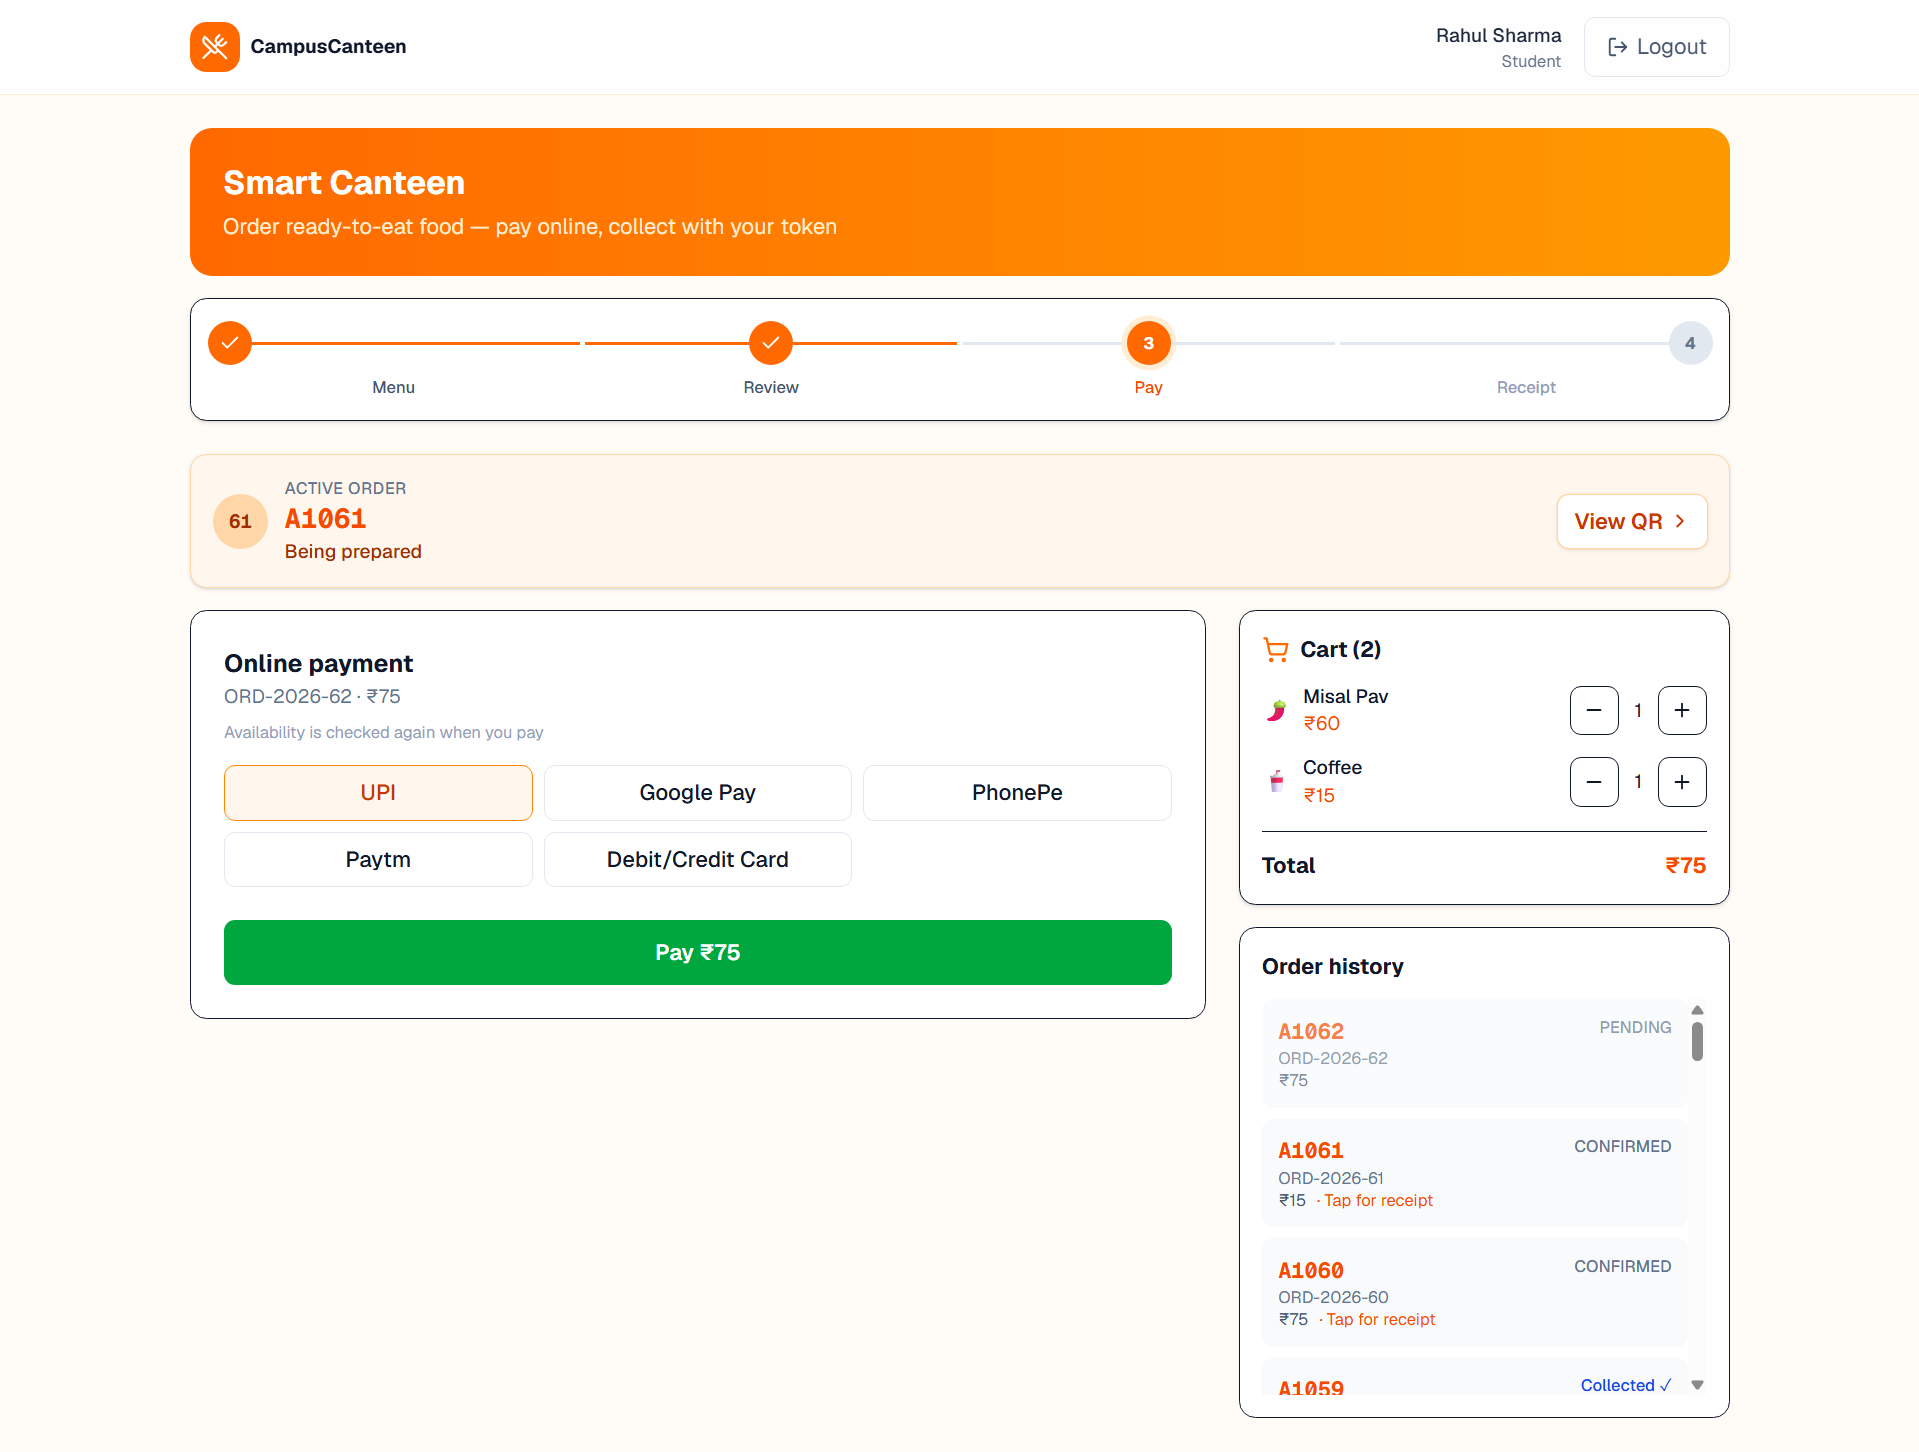
\includegraphics[width=0.85\textwidth]{images/04-payment.png}
  \caption{Payment confirmation screen}
  \label{fig:payment}
\end{figure}

\begin{figure}[htbp]
  \centering
  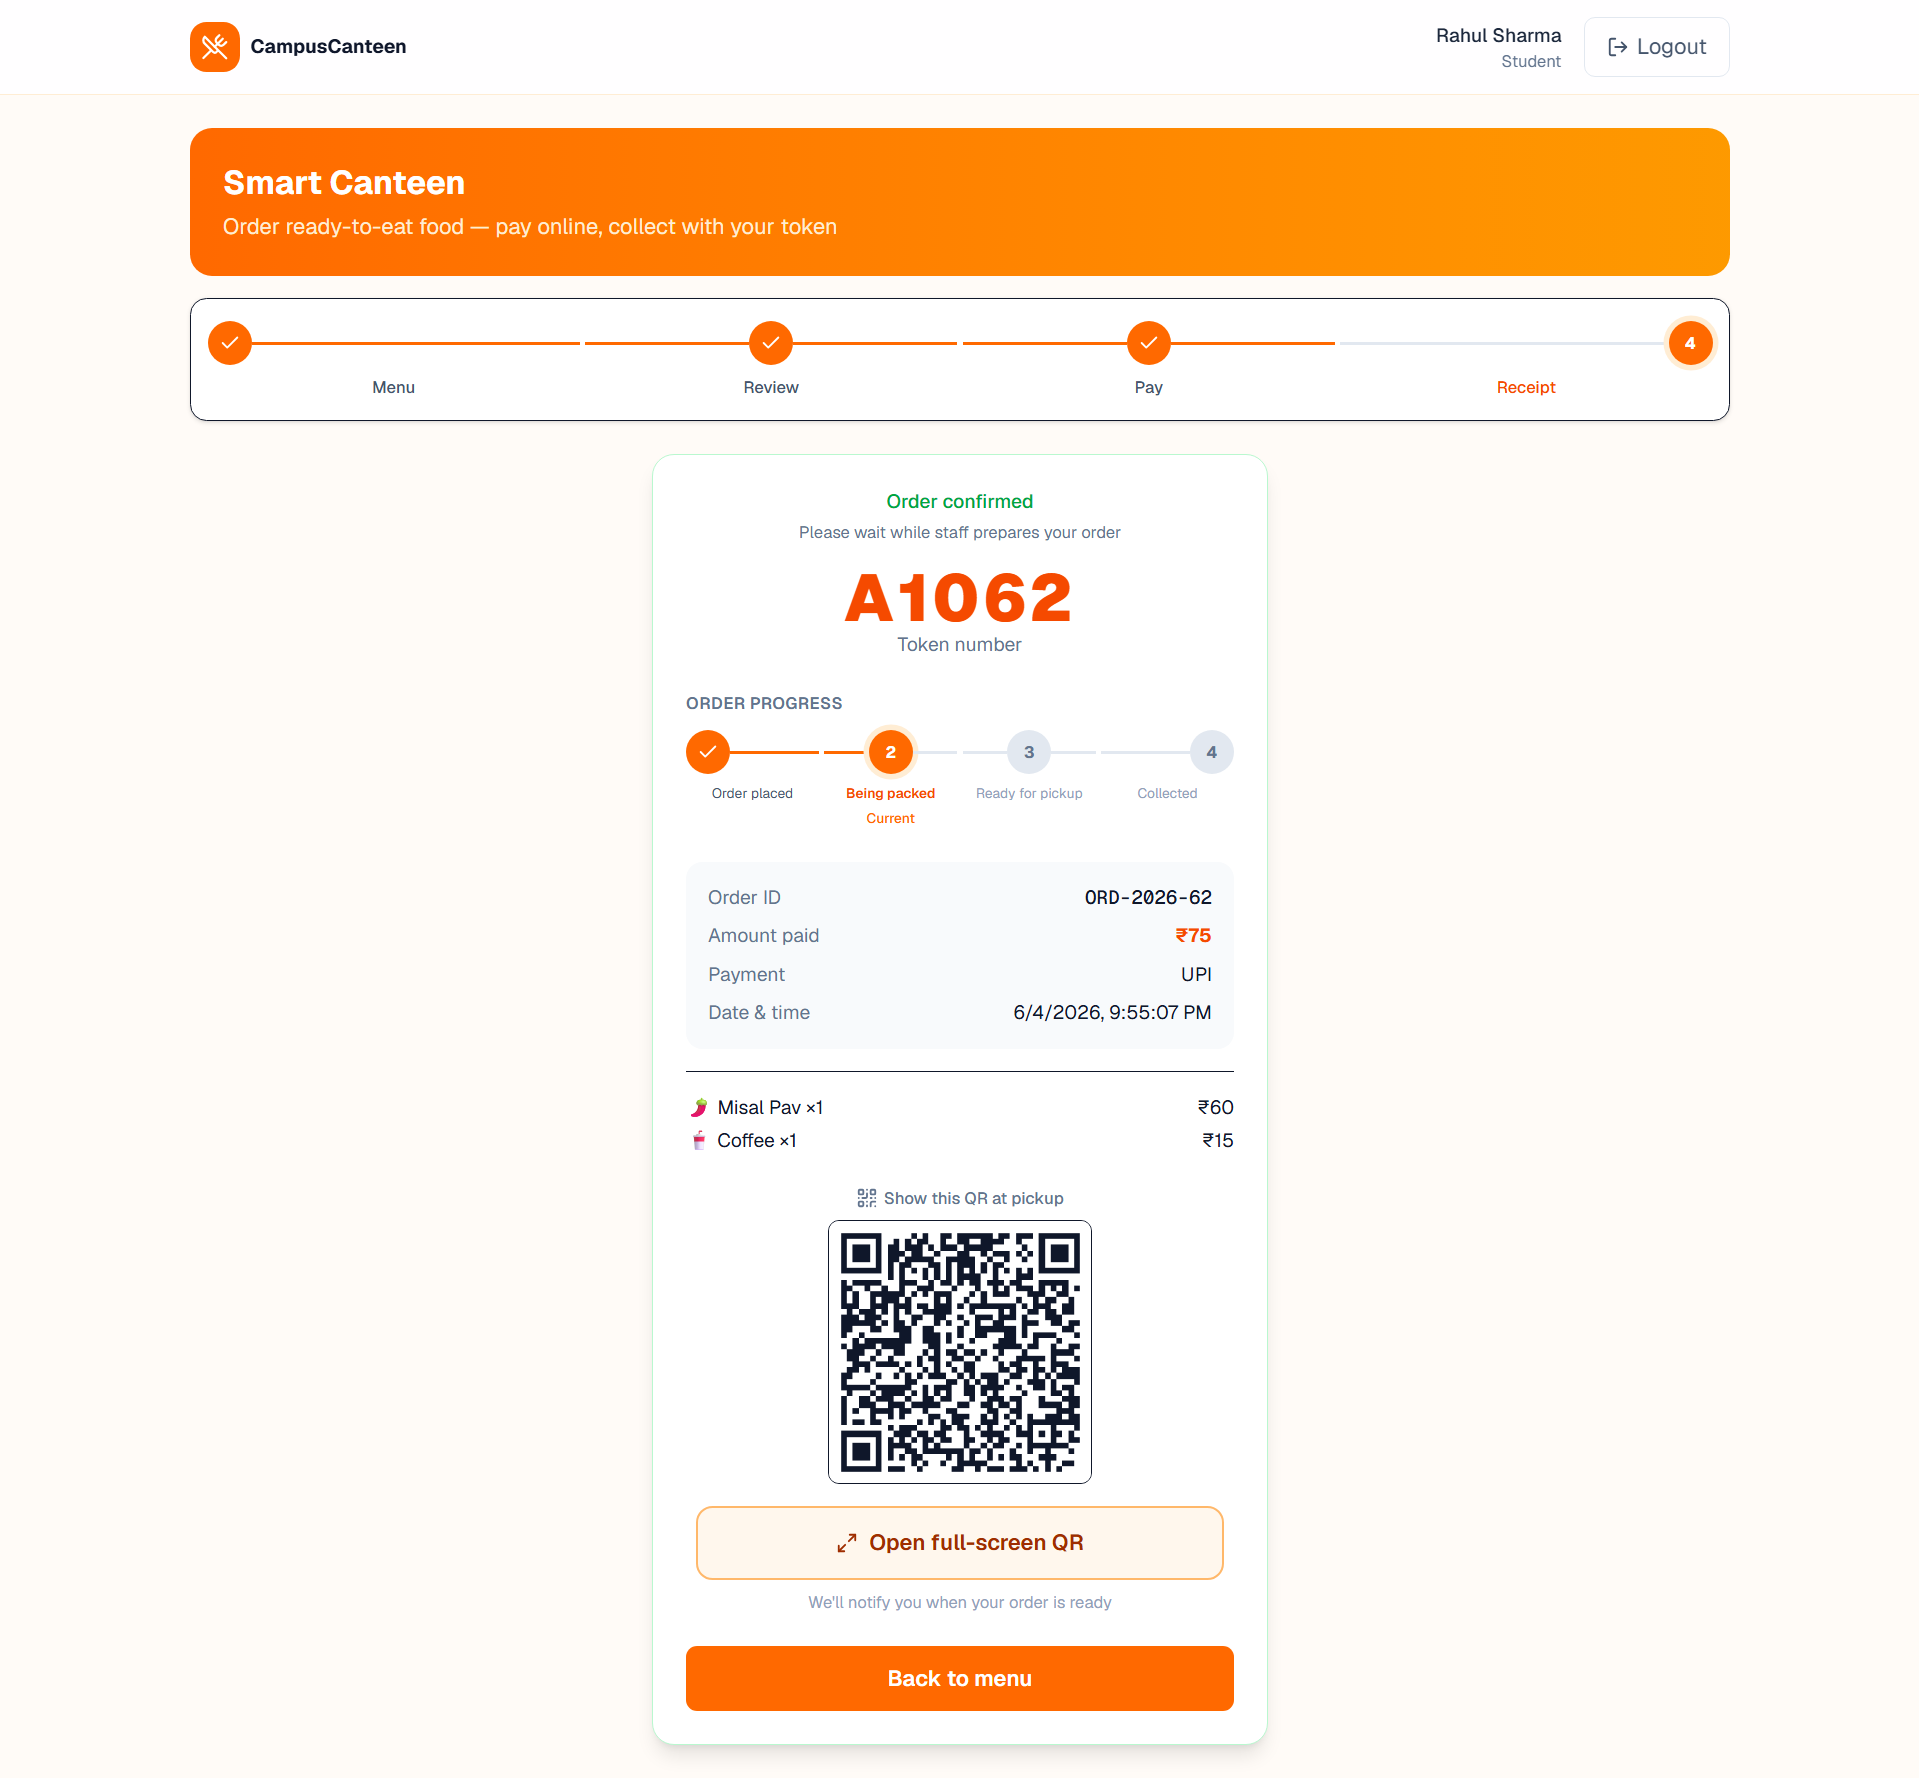
\includegraphics[width=0.85\textwidth]{images/05-receipt-qr.png}
  \caption{Order receipt with pickup token and QR code}
  \label{fig:receipt-qr}
\end{figure}

\begin{figure}[htbp]
  \centering
  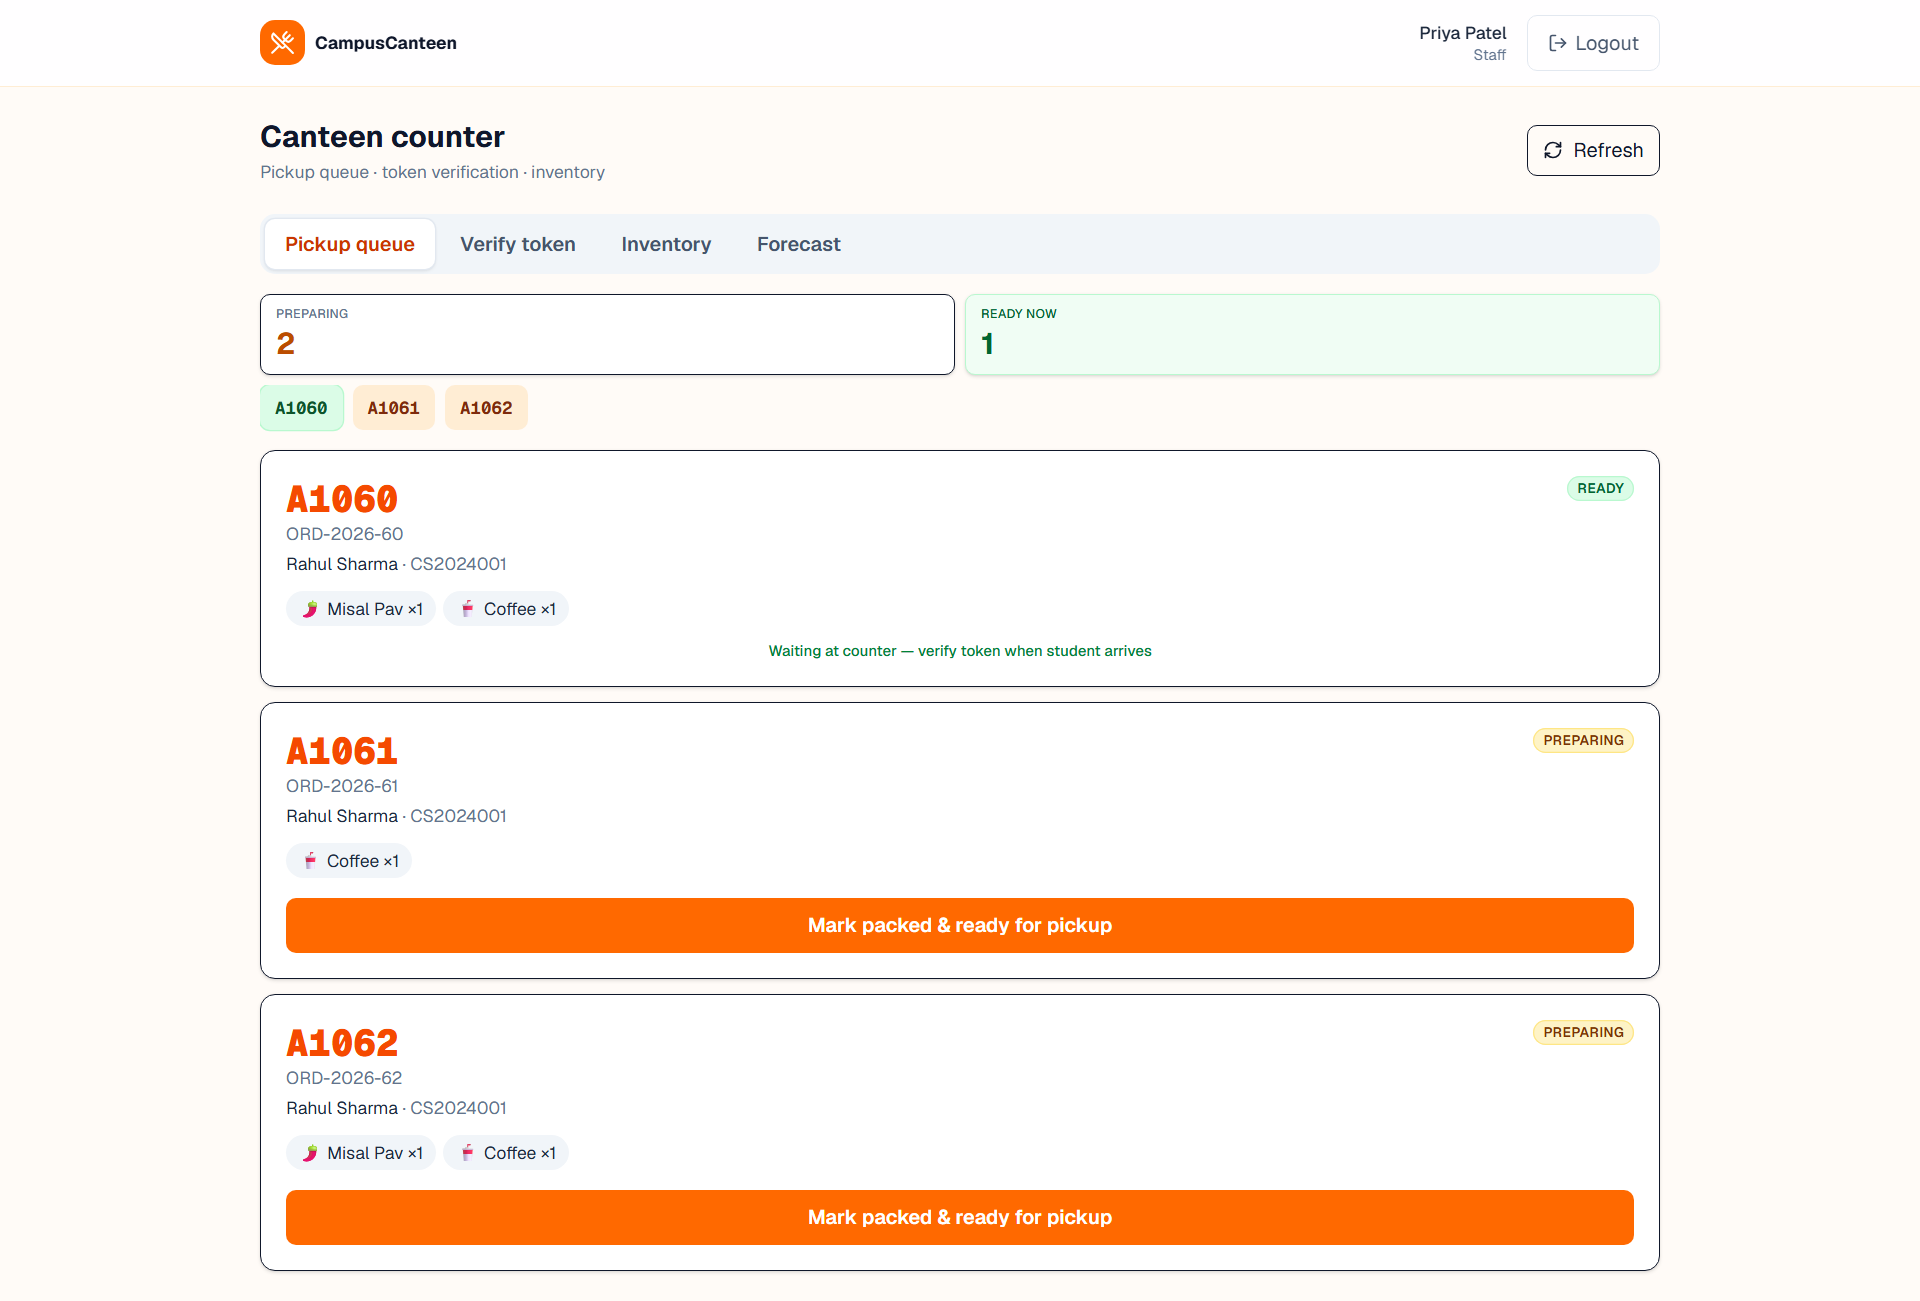
\includegraphics[width=0.85\textwidth]{images/06-student-orders.png}
  \caption{Student ``My orders'' tab with order status}
  \label{fig:student-orders}
\end{figure}

\begin{figure}[htbp]
  \centering
  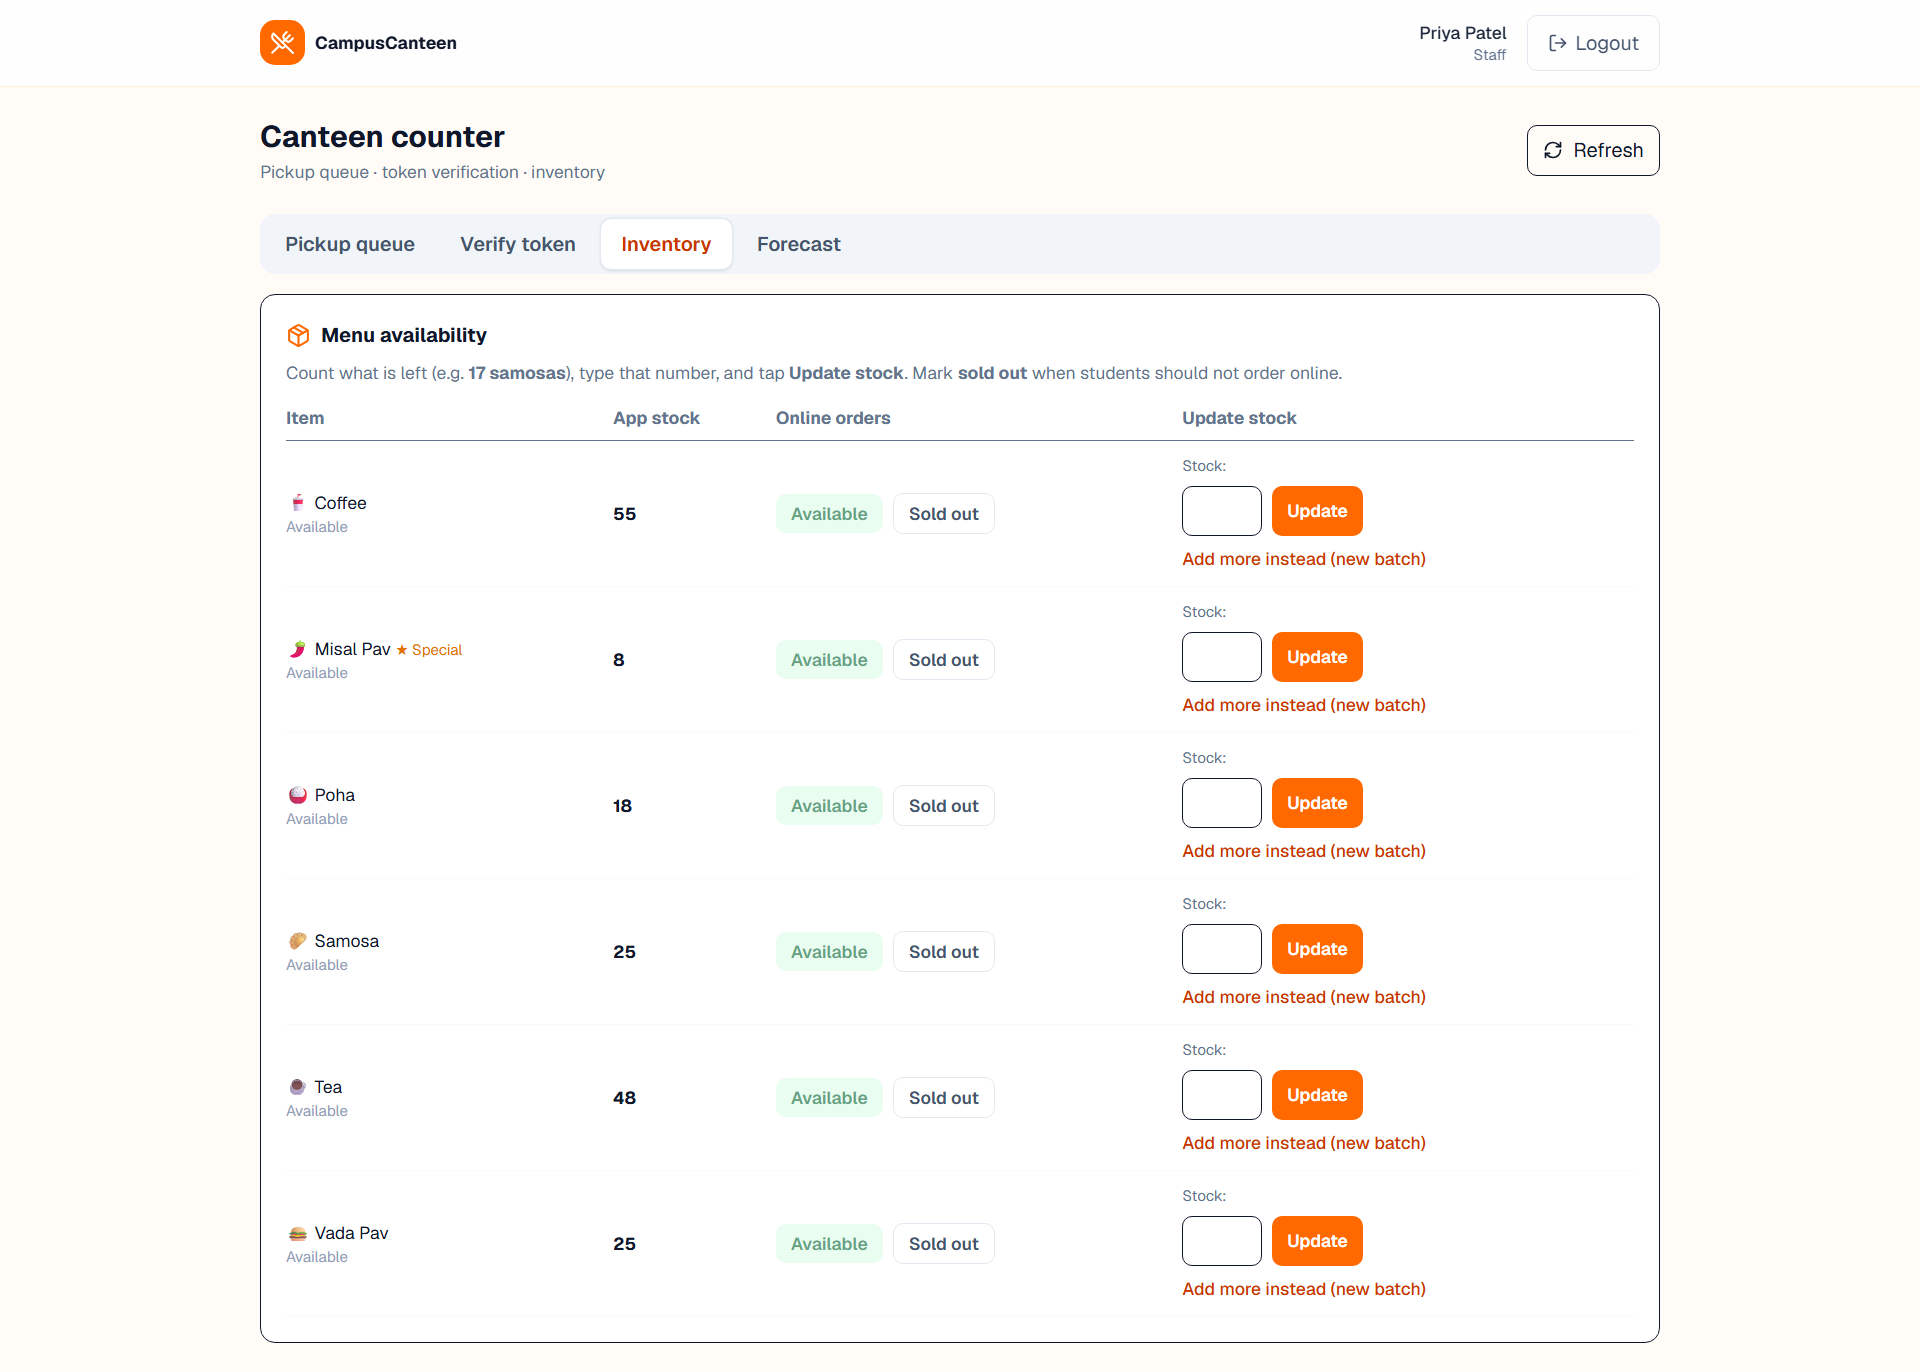
\includegraphics[width=0.85\textwidth]{images/07-staff-inventory.png}
  \caption{Staff inventory management with custom ``Set to'' stock (e.g.\ 17 samosas)}
  \label{fig:staff-inventory}
\end{figure}

\begin{figure}[htbp]
  \centering
  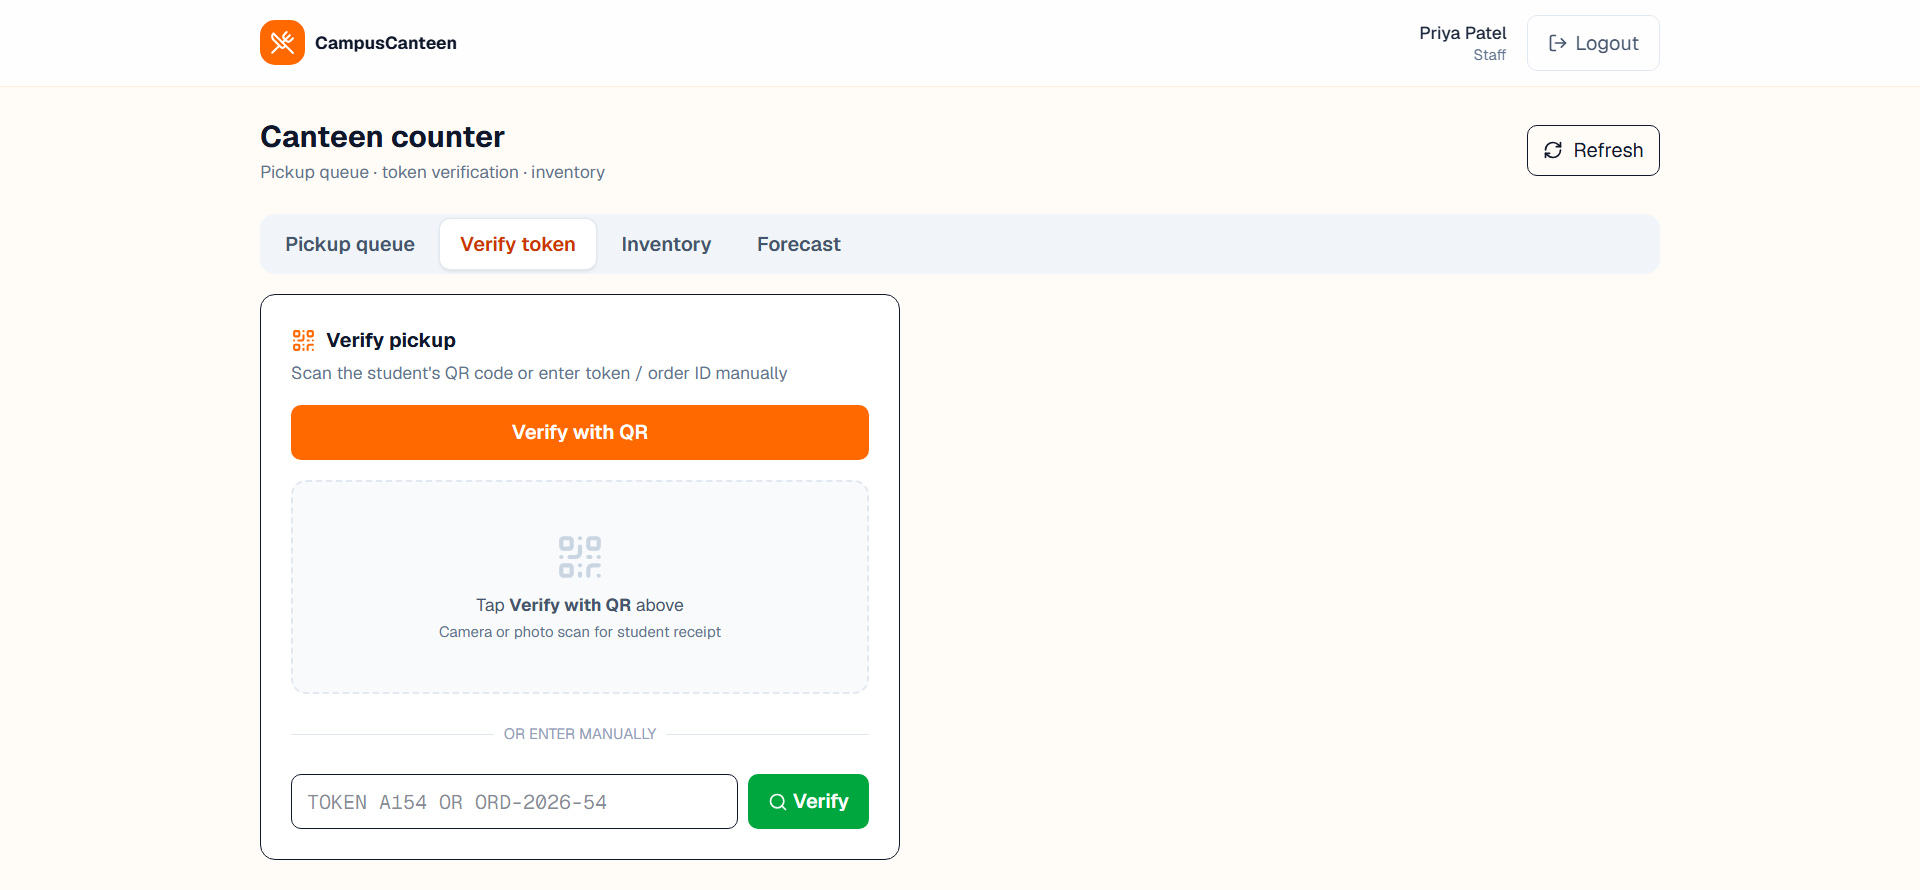
\includegraphics[width=0.85\textwidth]{images/08-staff-verify.png}
  \caption{Staff QR verification and handover screen}
  \label{fig:staff-verify}
\end{figure}

\else

\noindent\textcolor{red}{\textbf{[Screenshots not included yet.]}}
Add PNG files listed in Table~\ref{tab:screenshot-checklist} to the folder \texttt{images/}, then set \texttt{\textbackslash hasimagestrue} in \texttt{student-info.tex} and recompile twice so the List of Figures updates.

\fi


\section{Testing Approach}
Manual test cases are documented in Appendix~\ref{app:tests}. Testing included mobile viewport in Chrome DevTools, LAN access from Android phone, staff QR scan, and inventory update to arbitrary stock value.

\section{Version Control}
Project developed with Git. Recommended practice: commit after each milestone (auth, student flow, staff flow, mobile UI, inventory PATCH).

\chapter{Conclusion and Future Scope}

\section{Conclusion}
The \ShortTitle{} project delivers a complete software solution for inventory-aware canteen pre-ordering suited to college environments where food is prepared in batches. Students benefit from transparent stock information, streamlined payment, and QR-based pickup. Staff benefit from a structured queue, verification tools, custom inventory updates, and introductory demand forecasting.

The implementation demonstrates competence in full-stack web development: relational data modeling with Prisma, secure authentication, REST API design, mobile-first user experience, and integration of QR technology. The project aligns with the B.Tech Computer Engineering mini project objectives at Dr.\ Babasaheb Ambedkar Technological University, Lonere, including problem identification, literature review, structured design with DFD and UML diagrams, requirement analysis, coding, and testing documentation.

The choice of a progressive web application instead of a native Android app reduces development and maintenance cost while still supporting phone-based demonstration---a practical decision for academic scope and campus rollout.

\section{Achievements}
\begin{itemize}
  \item End-to-end student order-to-pickup flow with simulated payment.
  \item Multi-stage stock validation and post-payment stock deduction.
  \item Staff mobile workflow including QR scan and manual token entry.
  \item Custom inventory ``Set to N'' for real kitchen counts.
  \item Mobile-first UI with PWA install guidance.
  \item Comprehensive technical documentation and LaTeX project report.
\end{itemize}

\section{Limitations}
\begin{itemize}
  \item Payment gateway is simulated; no live UPI settlement.
  \item Cash counter sales require manual staff inventory updates.
  \item Cloud deployment prepared but deferred during report submission phase.
  \item Forecast accuracy limited without months of production data.
  \item No automated refund/cancel after payment in current version.
  \item Open registration may be unsuitable for public internet without hardening.
\end{itemize}

\section{Future Scope}
\begin{enumerate}
  \item \textbf{Production deployment:} Vercel + PostgreSQL (Neon), HTTPS, environment secrets, CI/CD pipeline.
  \item \textbf{Real payments:} Integrate Razorpay or PayU for UPI, cards, and receipts.
  \item \textbf{Operational policies:} Cancel/refund workflow with stock restoration and audit log.
  \item \textbf{Admin module:} Analytics dashboard, menu CRUD, staff account provisioning.
  \item \textbf{Notifications:} Web Push (VAPID) for reliable ``order ready'' alerts on iOS/Android.
  \item \textbf{Security:} Rate limiting, CAPTCHA on register, domain-restricted staff emails.
  \item \textbf{Forecasting:} Day-of-week features, special event tags, export CSV for kitchen.
  \item \textbf{Hardware:} Optional thermal printer for token slip backup if QR fails.
\end{enumerate}

\section{Closing Remarks}
\ShortTitle{} shows that a well-designed web application can address real campus canteen pain points without immediate investment in native mobile development. Continued work should focus on trustworthy payments, production hosting, and day-to-day staff discipline in stock updates so the digital inventory reflects the physical counter.

\begin{thebibliography}{99}
\addcontentsline{toc}{chapter}{Bibliography}

\bibitem{nextjs}
Vercel Inc.\ (2024).
\newblock \emph{Next.js Documentation}.
\newblock \url{https://nextjs.org/docs} (accessed 2026).

\bibitem{prisma}
Prisma Data Inc.\ (2024).
\newblock \emph{Prisma ORM Documentation}.
\newblock \url{https://www.prisma.io/docs} (accessed 2026).

\bibitem{pwa}
Mozilla Developer Network (2024).
\newblock \emph{Progressive Web Apps}.
\newblock \url{https://developer.mozilla.org/en-US/docs/Web/Progressive_web_apps} (accessed 2026).

\bibitem{qr}
ISO/IEC 18004:2015.
\newblock \emph{Information technology --- Automatic identification and data capture techniques --- QR Code bar code symbology specification}.

\bibitem{uml}
Object Management Group (2017).
\newblock \emph{Unified Modeling Language Specification, Version 2.5.1}.

\bibitem{forecast}
Hyndman, R.\ J., and Athanasopoulos, G.\ (2021).
\newblock \emph{Forecasting: Principles and Practice}, 3rd ed.
\newblock OTexts. \url{https://otexts.com/fpp3/}.

\bibitem{batu}
Dr.\ Babasaheb Ambedkar Technological University, Lonere.
\newblock Department of Computer Engineering --- B.Tech Project Report Format Guidelines.

\bibitem{jwt}
Jones, M., Bradley, J., and Sakimura, N.\ (2015).
\newblock JSON Web Token (JWT).
\newblock RFC 7519, IETF.

\end{thebibliography}


\end{document}
